\chapter{SELEÇÃO, CARACTERIZAÇÃO E PREPARAÇÃO DOS DATASETS}

\section{Critérios de seleção}

A passagem dos cenários gaussianos idealizados para experimentos ancorados em dados reais exigiu mais do que a escolha de bases públicas com número suficiente de linhas. O protocolo demanda que cada variável selecionada possa ser interpretada como um canal de informação, que o alvo possua significado defensável no domínio, que o número de canais permita a enumeração exaustiva dos subconjuntos não vazios e que seja possível construir uma separação entre treinamento e teste compatível com a dependência presente nos dados. Também se exigiu que todas as operações dependentes dos dados --- definição de limiar, padronização, parametrização dos geradores e calibração dos classificadores --- fossem executadas sem acesso ao conjunto de teste.

Esses critérios são importantes porque a disponibilidade pública de um arquivo tabular não garante que suas linhas possam ser tratadas como observações independentes. Vazamento de informação pode ocorrer quando variáveis relacionadas ao desfecho, etapas de pré-processamento ou observações correlacionadas aparecem simultaneamente no treinamento e na avaliação \cite{Kaufman2012}. Em dados com estrutura temporal, espacial, hierárquica ou por grupos, divisões aleatórias podem produzir estimativas excessivamente otimistas; nesses casos, a estratégia de validação deve representar a forma de generalização de interesse \cite{Roberts2017,Bergmeir2012}.

Foram priorizados problemas binários de pequena ou média dimensionalidade, com canais fisicamente ou semanticamente interpretáveis e reservatórios de treinamento capazes de sustentar amostragem balanceada em diferentes valores de $n$. A dimensionalidade foi deliberadamente mantida baixa: com $d$ canais, o número de subconjuntos não vazios é $2^d-1$, de modo que o custo do experimento cresce exponencialmente antes mesmo de considerar classificadores, braços, tamanhos amostrais e replicações.

\section{Datasets considerados e não incorporados}

\subsection{CSI Wi-Fi}

Dados de informação de estado do canal em redes Wi-Fi foram considerados por representarem um exemplo natural de múltiplos canais de informação. Entretanto, as observações costumam estar organizadas por indivíduo, sessão, posição, ambiente ou janela temporal. Uma divisão aleatória de linhas poderia colocar no treinamento e no teste medições muito próximas ou provenientes da mesma realização física, permitindo que o classificador explorasse dependências específicas da sessão em vez de generalizar para novas condições.

A incorporação desse tipo de dado exigiria definir previamente a unidade amostral, a política de agrupamento e o regime de generalização: novas janelas da mesma sessão, novas sessões do mesmo indivíduo, novos indivíduos ou novos ambientes. Como essa modelagem excedia o escopo temporal do presente trabalho, o dataset não foi tratado como uma tabela de linhas independentes. A decisão segue as recomendações de validação estruturada para dados temporal e hierarquicamente dependentes \cite{Roberts2017,Bergmeir2012}.

\subsection{Sistema hidráulico industrial}

Também foi estudada a possibilidade de utilizar dados de monitoramento de um sistema hidráulico industrial. Nesse domínio, diferentes sensores registram séries durante ciclos operacionais, e o alvo pode representar falhas ou condições do equipamento. Apesar da aderência à motivação de custo e seleção de sensores, a transformação de séries e ciclos em observações classificáveis requer decisões próprias: agregação temporal, segmentação, independência entre ciclos e separação por período ou regime operacional.

O dataset permanece relevante para trabalhos futuros, mas sua inclusão no protocolo atual exigiria uma extensão explícita para dados dependentes no tempo. O adiamento evita que uma sequência temporal seja artificialmente tratada como um conjunto tabular independente e reduz o risco de vazamento entre ciclos correlacionados \cite{Kaufman2012,Roberts2017}.

\section{Occupancy Detection}

\subsection{Origem e finalidade}

O dataset \textit{Occupancy Detection}, disponibilizado no UCI Machine Learning Repository sob o DOI \texttt{10.24432/C5X01N}, foi apresentado por \textcite{candanedo2016} para detectar a ocupação de uma sala a partir de medições ambientais. O rótulo binário foi obtido por fotografias com marcação temporal, enquanto os canais registram temperatura, umidade relativa, luminosidade, concentração de dióxido de carbono e razão de umidade. O conjunto também foi empregado posteriormente em estudos de séries multivariadas e detecção de ocupação \cite{Wu2019}; trabalhos relacionados investigaram ainda transferência a partir de dados ambientais sintéticos para reduzir a necessidade de coleta real \cite{Weber2020}.

O cenário utiliza cinco canais:

\begin{enumerate}[label=$X_{\arabic*}$:]
  \item \texttt{Temperature}, em graus Celsius;
  \item \texttt{Humidity}, em porcentagem;
  \item \texttt{Light}, em lux;
  \item \texttt{CO2}, em partes por milhão;
  \item \texttt{HumidityRatio}, razão entre massa de água e massa de ar.
\end{enumerate}

O alvo \texttt{Occupancy} assume 0 para sala desocupada e 1 para sala ocupada. Com cinco canais, o experimento avalia os 31 subconjuntos não vazios.

\subsection{Particionamento e preparação}

Foi preservada a divisão distribuída com o dataset. O arquivo \texttt{datatraining.txt}, com 8.143 linhas, constitui o reservatório finito de treinamento. Os arquivos \texttt{datatest.txt} e \texttt{datatest2.txt}, com 2.665 e 9.752 linhas, respectivamente, são concatenados para formar um teste real fixo com 12.417 observações. No reservatório de treinamento, as classes 0 e 1 possuem 6.414 e 1.729 registros. No teste combinado, os totais correspondentes são 9.396 e 3.021.

A média e o desvio-padrão de cada canal são estimados exclusivamente no reservatório de treinamento, usando desvio populacional ($\mathrm{ddof}=0$), e aplicados aos dois conjuntos. Não há imputação, e os arquivos empregados não apresentam valores ausentes nas colunas obrigatórias. A amostragem Monte Carlo do braço real é balanceada, sem reposição dentro de cada replicação, sendo seu maior $n$ limitado pela classe minoritária do reservatório.

\subsection{Geometria observada}

A inspeção das projeções padronizadas mostra classes com formas irregulares, concentrações alongadas e regiões cuja geometria se distancia de uma única elipse gaussiana. Essa característica torna o cenário especialmente informativo: a Gaussiana única produz pontos visualmente muito diferentes dos dados reais, enquanto o GMM acompanha melhor parte da forma empírica. Ainda assim, como será discutido nos resultados, fidelidade visual e fidelidade estrutural não coincidem necessariamente. No maior $n$, a Gaussiana única pode apresentar correlação de ranking e \WinnersAgreement{} ligeiramente superiores às do GMM, mesmo quando o GMM parece imitar melhor a nuvem real. A Figura~\ref{fig:geom-occupancy-dataset} apresenta as projeções bidimensionais padronizadas dos três braços, extraídas do relatório do cenário 000002.

\begin{figure}[H]
  \centering
  \caption{Geometrias padronizadas do cenário Occupancy Detection}
  \label{fig:geom-occupancy-dataset}
  \begin{minipage}{\textwidth}
    \centering
    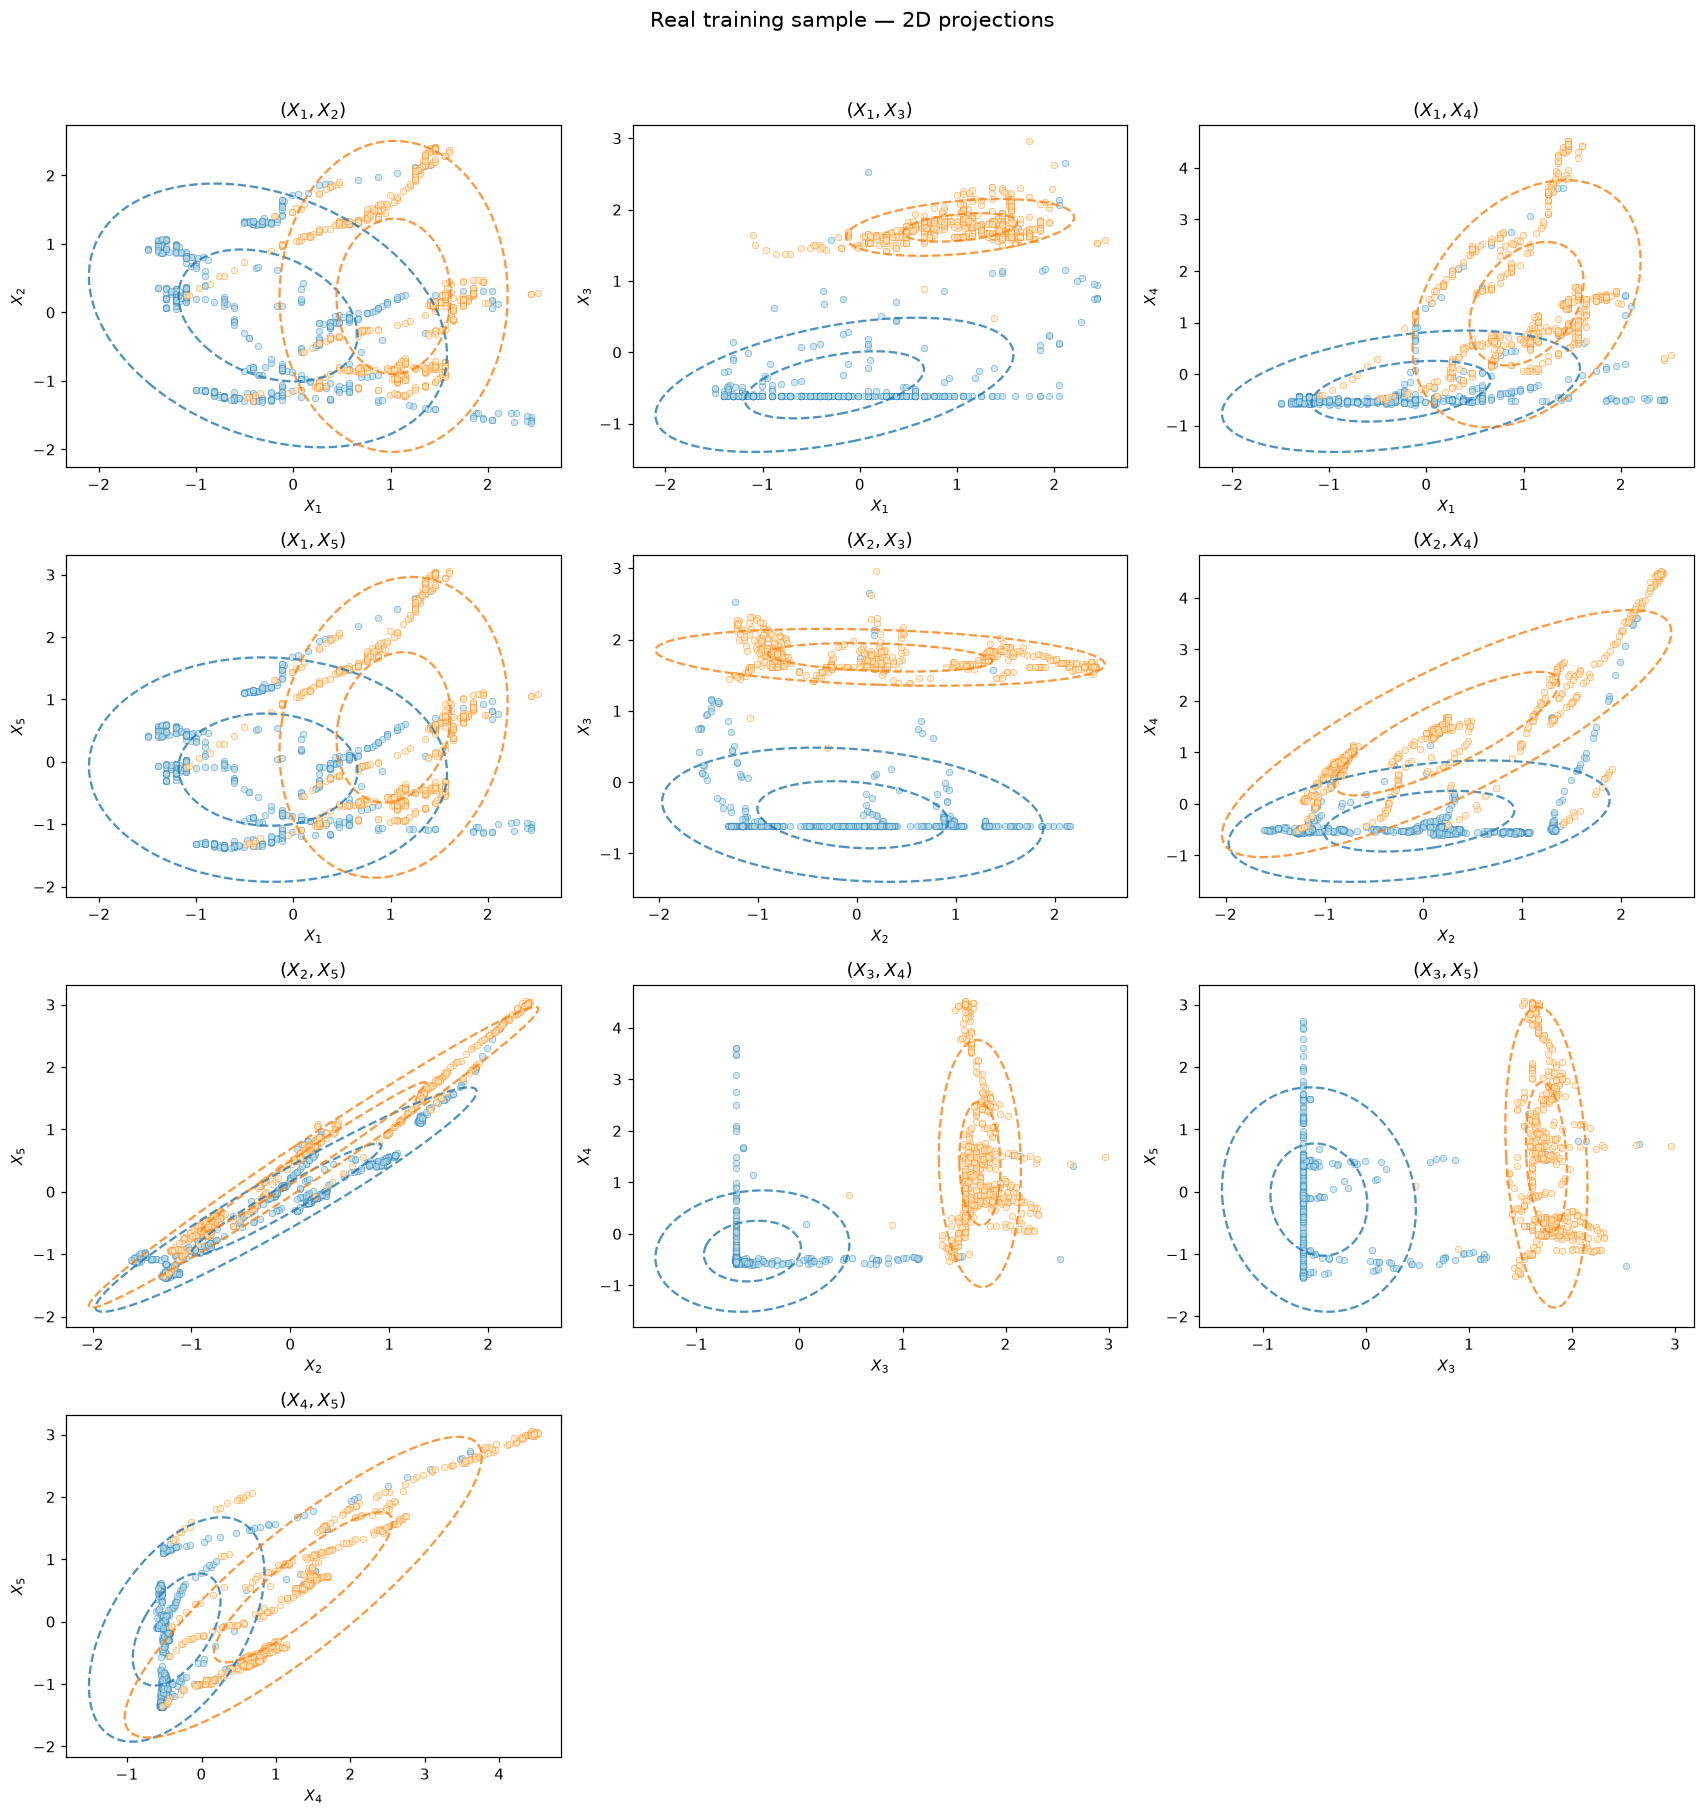
\includegraphics[width=\textwidth,height=0.82\textheight,keepaspectratio]{figures/geometry/occupancy/viz_2d_real_full_000002.png}
    \subcaption{Dados reais}
  \end{minipage}
  \sourcebelow{relatório publicado do cenário Occupancy Detection 000002 do \CoInfoSim}
\end{figure}

\begin{figure}[H]
  \ContinuedFloat
  \centering
  \caption[]{Geometrias padronizadas do cenário Occupancy Detection (continuação)}
  \begin{minipage}{\textwidth}
    \centering
    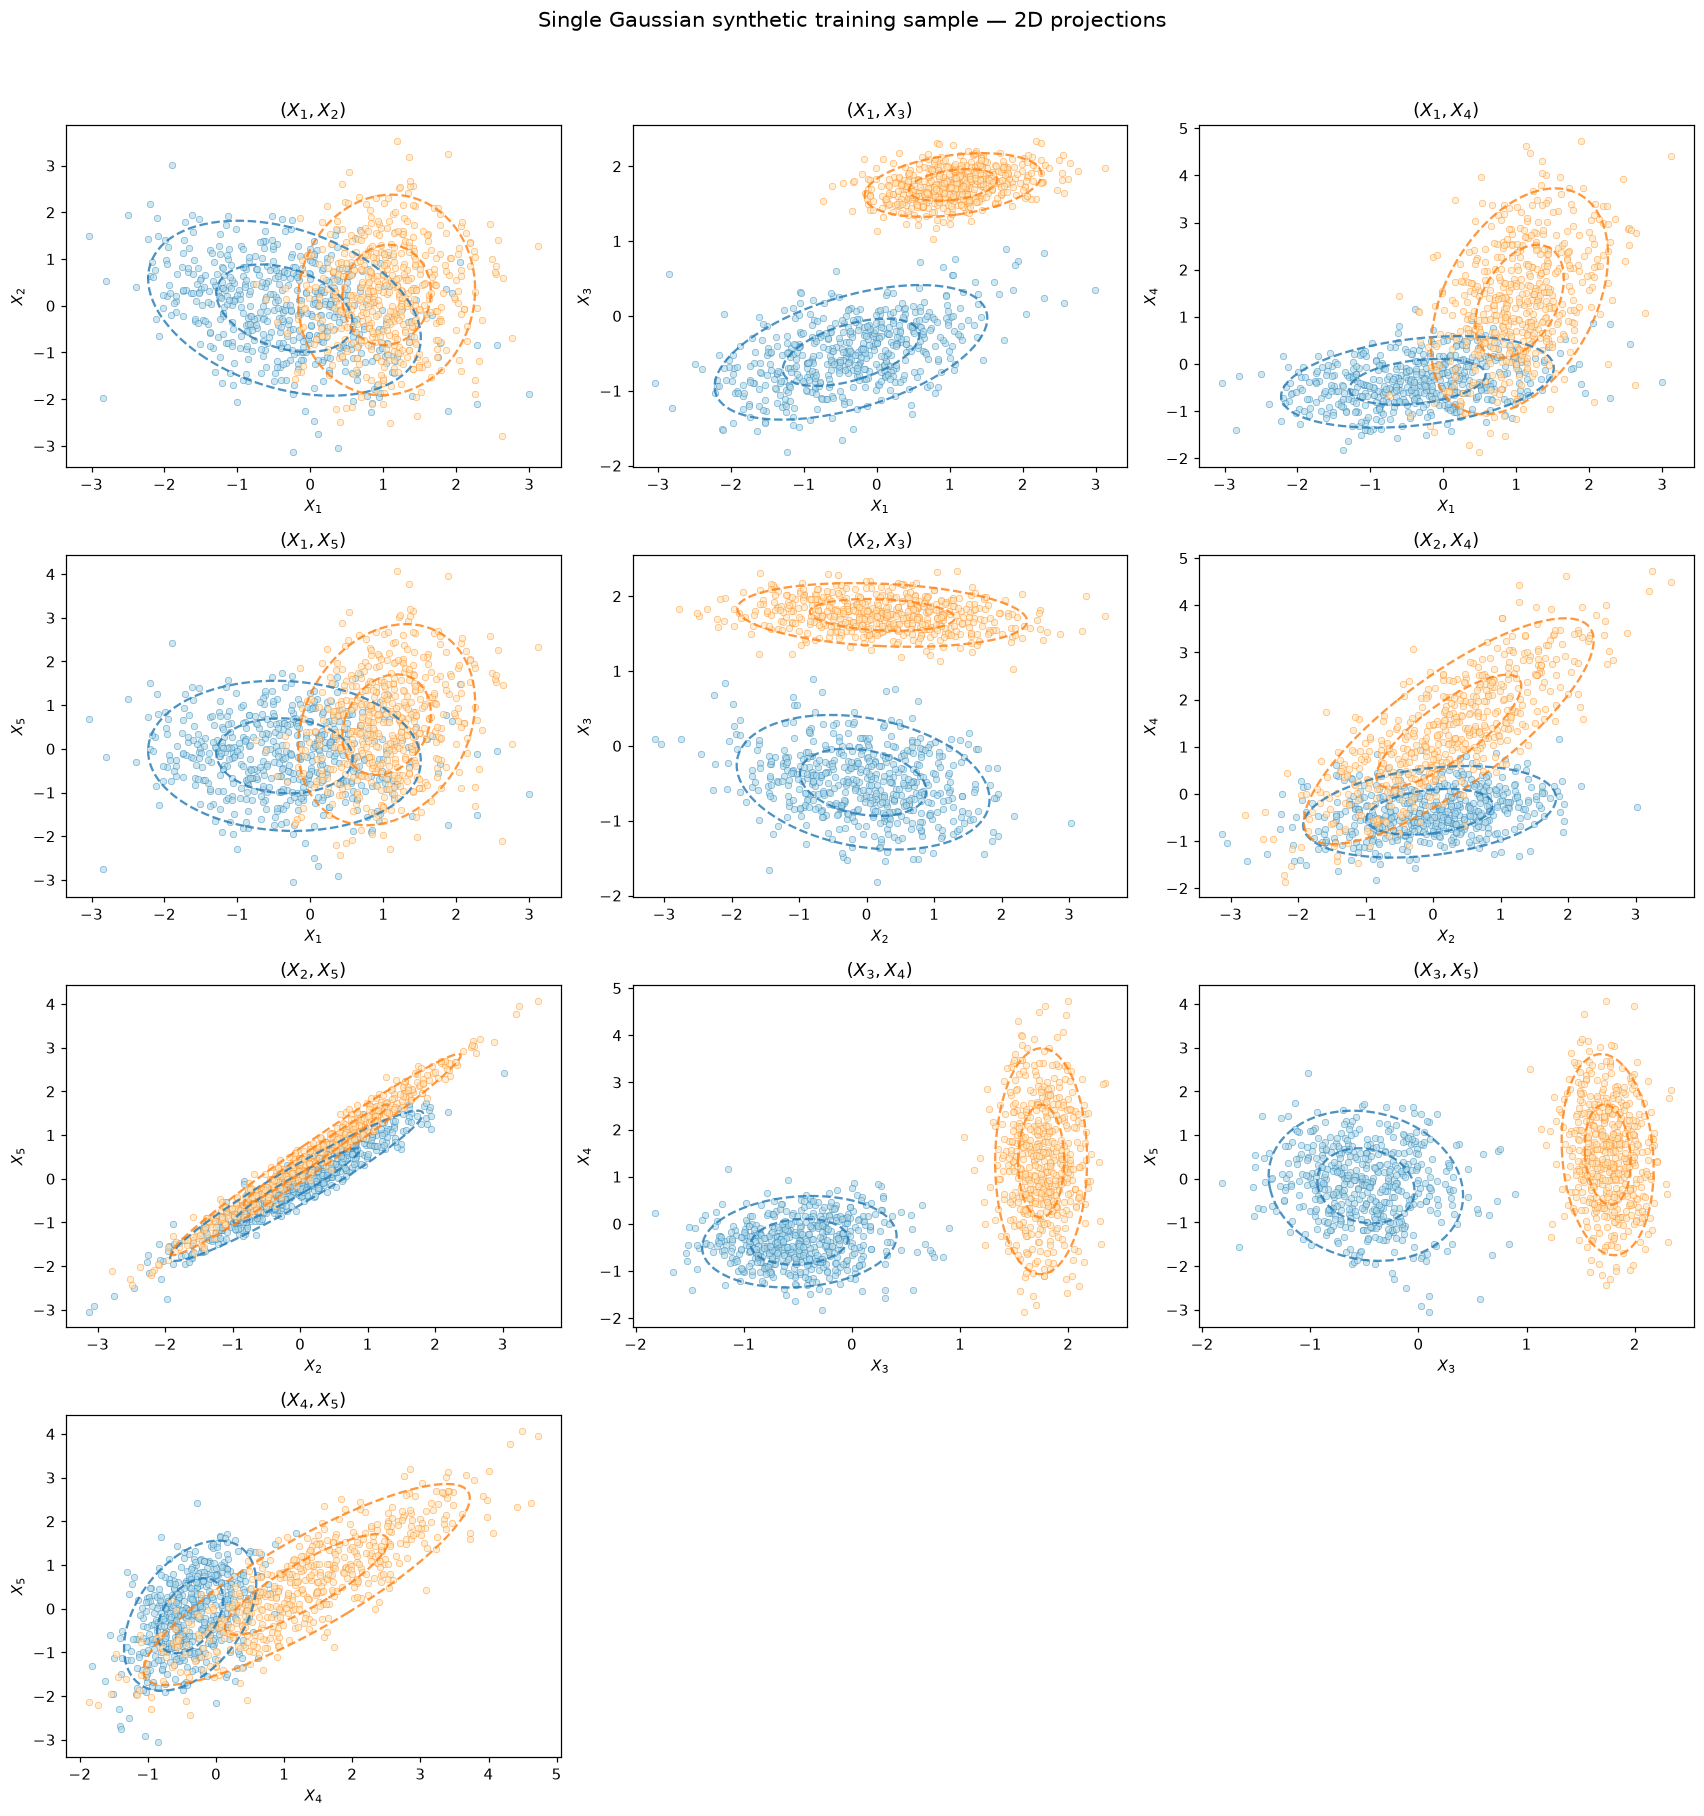
\includegraphics[width=\textwidth,height=0.82\textheight,keepaspectratio]{figures/geometry/occupancy/viz_2d_gaussian_full_000002.png}
    \subcaption{Gaussiana única}
  \end{minipage}
  \sourcebelow{relatório publicado do cenário Occupancy Detection 000002 do \CoInfoSim}
\end{figure}

\begin{figure}[H]
  \ContinuedFloat
  \centering
  \caption[]{Geometrias padronizadas do cenário Occupancy Detection (continuação)}
  \begin{minipage}{\textwidth}
    \centering
    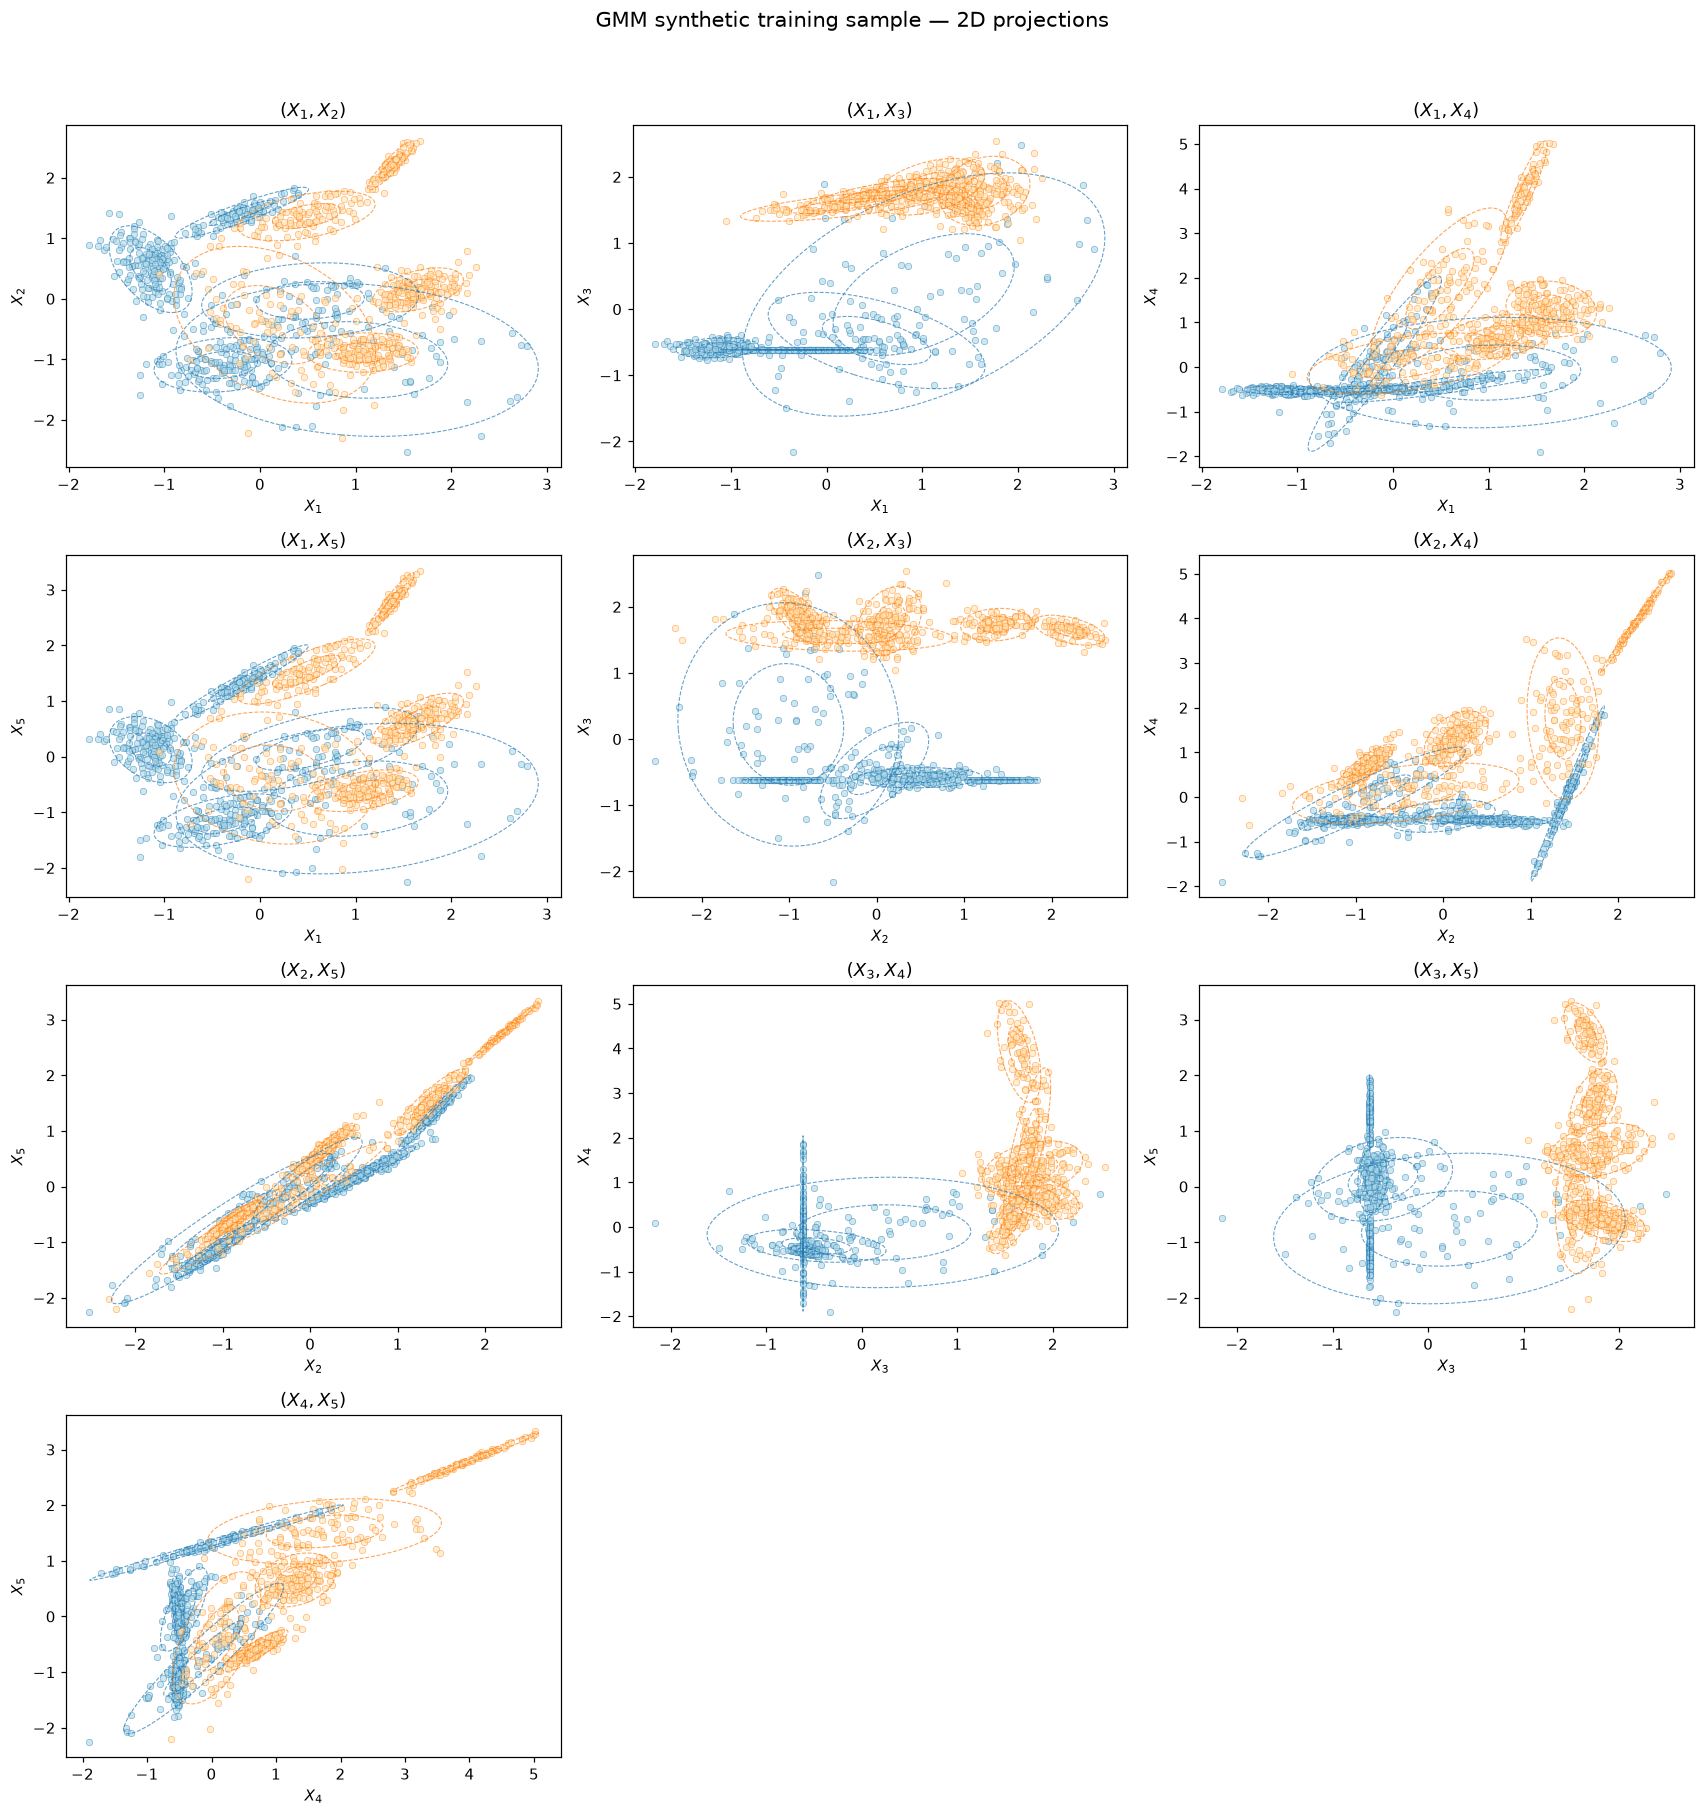
\includegraphics[width=\textwidth,height=0.82\textheight,keepaspectratio]{figures/geometry/occupancy/viz_2d_gmm_full_000002.png}
    \subcaption{GMM}
  \end{minipage}
  \sourcebelow{relatório publicado do cenário Occupancy Detection 000002 do \CoInfoSim}
  \notailustracao{A comparação geométrica é descritiva. A preservação estrutural é avaliada separadamente pelas métricas definidas no Capítulo 6.}
\end{figure}

\section{UCI Air Quality}

\subsection{Origem e natureza dos canais}

O dataset \textit{Air Quality}, UCI 360, DOI \texttt{10.24432/C59K5F}, reúne respostas horárias de um dispositivo multissensor instalado em ambiente urbano. O estudo associado investigou a calibração em campo de um nariz eletrônico para estimação de benzeno \cite{devito2008}. Os canais PT08 são respostas elétricas de sensores de óxido metálico nominalmente associados a determinados gases; eles não devem ser interpretados como cinco medições independentes de concentração, pois apresentam sensibilidade cruzada, envelhecimento e deriva. O conjunto permanece utilizado em pesquisas de extração de padrões temporais \cite{Jang2018} e em avaliações recentes de modelos leves para monitoramento embarcado \cite{Sami2025}.

Foram selecionados os cinco canais de resposta:

\begin{enumerate}[label=$X_{\arabic*}$:]
  \item \texttt{PT08.S1(CO)};
  \item \texttt{PT08.S2(NMHC)};
  \item \texttt{PT08.S3(NOx)};
  \item \texttt{PT08.S4(NO2)};
  \item \texttt{PT08.S5(O3)}.
\end{enumerate}

A variável \texttt{C6H6(GT)}, obtida por analisador de referência, não é fornecida ao classificador. Ela é usada somente para construir o alvo binário \texttt{benzene\_elevated}. Assim, o problema representa a tentativa de inferir uma condição definida por equipamento de referência a partir de sensores potencialmente mais simples. O limiar experimental não constitui limite sanitário ou regulatório.

\subsection{Coorte, alvo e divisão cronológica}

O arquivo possui 9.357 linhas não vazias. O valor sentinela $-200$ é convertido em ausente, e são mantidas apenas as observações completas nos cinco canais e na referência de benzeno. A coorte resultante contém 8.991 linhas; 366 observações são descartadas, sem imputação.

Depois da ordenação temporal, as primeiras 7.192 observações, correspondentes a 80\% da coorte, formam o reservatório de treinamento; as 1.799 observações posteriores formam o teste real fixo. O treinamento cobre o período de 10 de março de 2004, às 18h, até 16 de janeiro de 2005, à 1h. O teste começa imediatamente depois, às 2h, e termina em 4 de abril de 2005, às 14h. Esse corte preserva uma tarefa de generalização para observações futuras e impede que medições posteriores participem da parametrização dos geradores.

O limiar do alvo é o percentil 75 da referência \texttt{C6H6(GT)} calculado somente no treinamento, igual a 14,5 na preparação atual. A classe positiva satisfaz \texttt{C6H6(GT) >= 14.5}. O treinamento contém 5.374 negativos e 1.818 positivos; o teste, 1.524 negativos e 275 positivos. Os parâmetros de padronização são estimados apenas no treinamento e aplicados ao teste.

\subsection{Geometria observada}

As projeções do Air Quality apresentam regiões mais compactas e elipsoidais do que as observadas no Occupancy, embora não sejam perfeitamente gaussianas. A maior regularidade fornece um contraste útil para investigar quando uma única Gaussiana já retém informação estrutural suficiente e quando os componentes adicionais do GMM modificam as relações entre subconjuntos. A Figura~\ref{fig:geom-air-dataset} apresenta as projeções bidimensionais dos cinco sensores nos três braços, com as classes definidas pela referência de benzeno.

\begin{figure}[H]
  \centering
  \caption{Geometrias padronizadas do cenário UCI Air Quality}
  \label{fig:geom-air-dataset}
  \begin{minipage}{\textwidth}
    \centering
    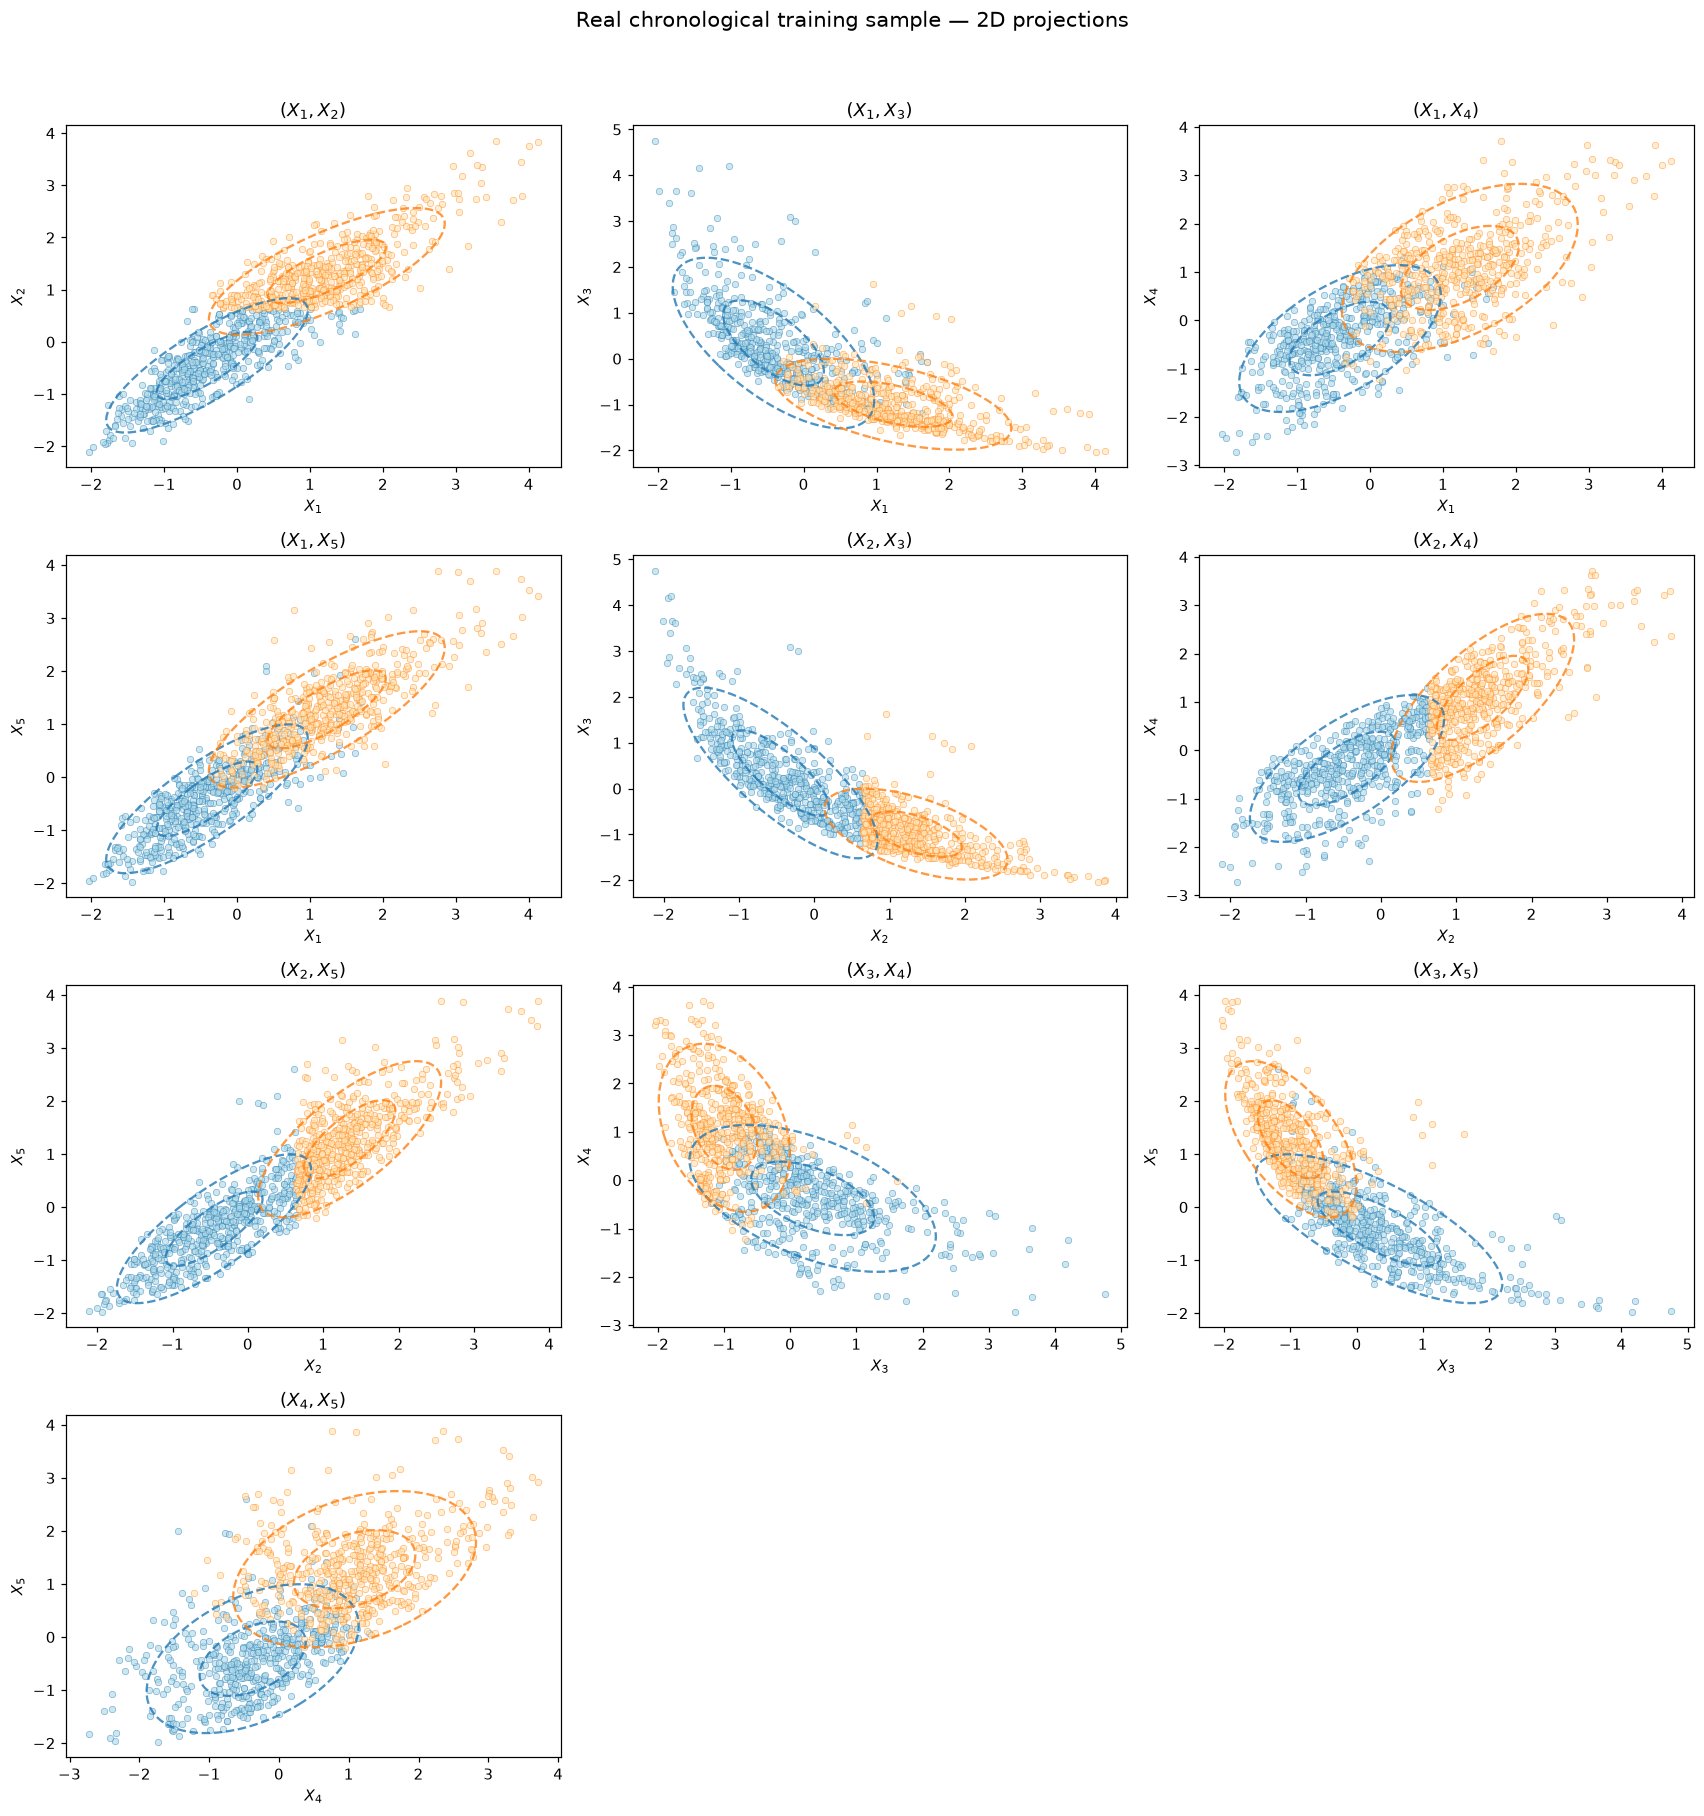
\includegraphics[width=\textwidth,height=0.82\textheight,keepaspectratio]{figures/geometry/air_quality/viz_2d_real_full_000005.png}
    \subcaption{Dados reais}
  \end{minipage}
  \sourcebelow{relatório publicado do cenário Air Quality 000005 do \CoInfoSim}
\end{figure}

\begin{figure}[H]
  \ContinuedFloat
  \centering
  \caption[]{Geometrias padronizadas do cenário UCI Air Quality (continuação)}
  \begin{minipage}{\textwidth}
    \centering
    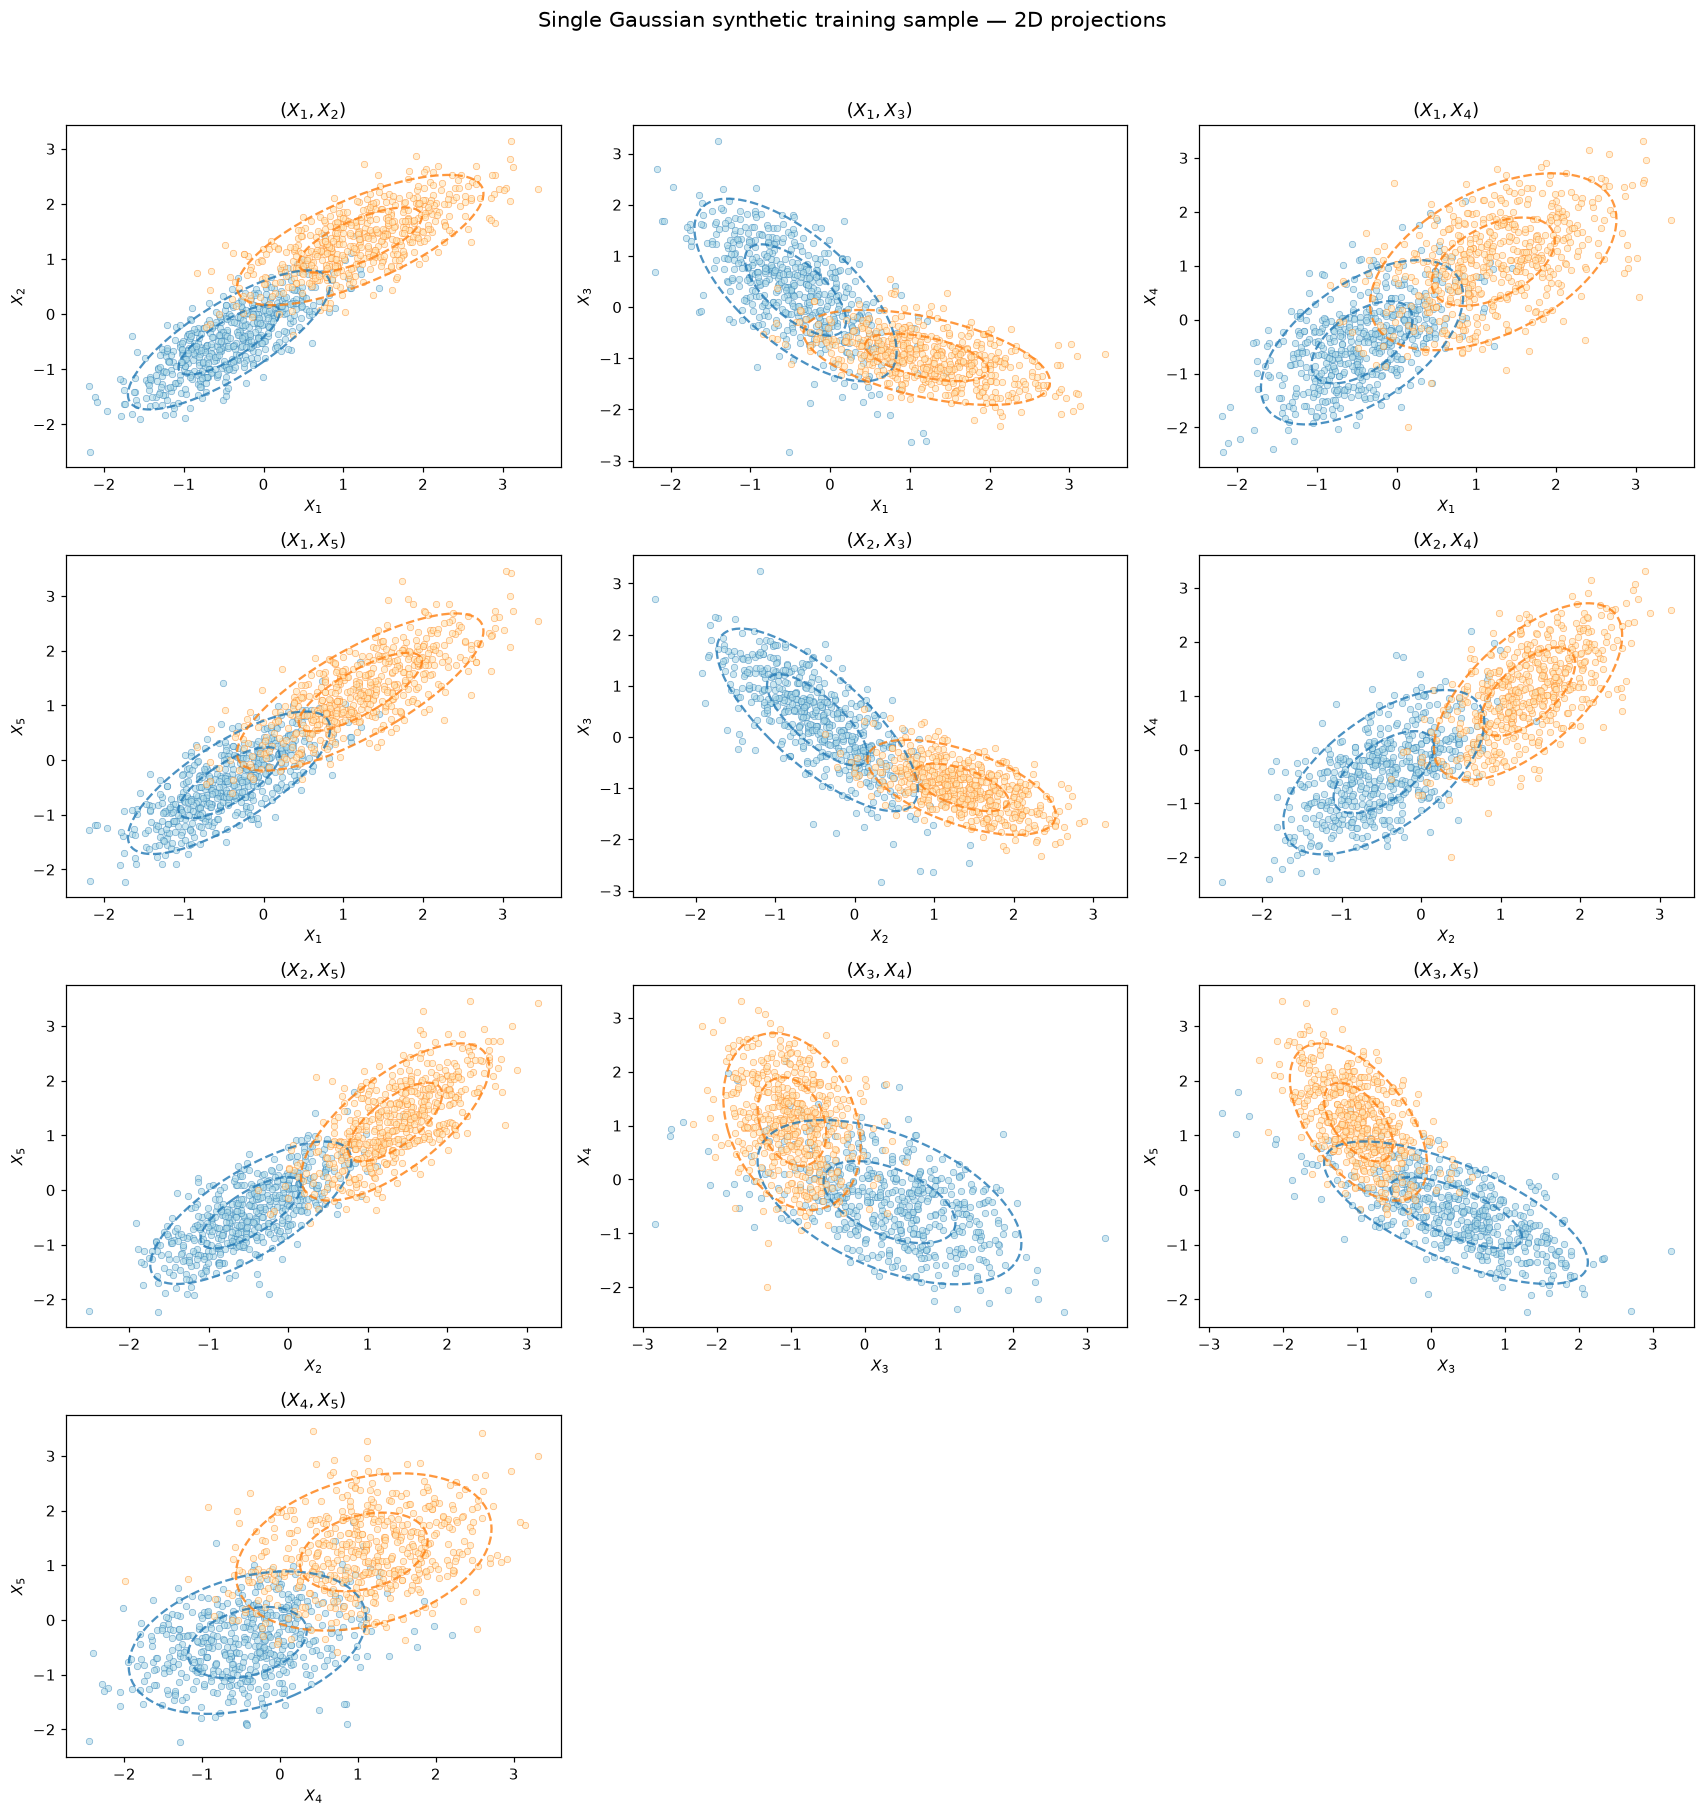
\includegraphics[width=\textwidth,height=0.82\textheight,keepaspectratio]{figures/geometry/air_quality/viz_2d_gaussian_full_000005.png}
    \subcaption{Gaussiana única}
  \end{minipage}
  \sourcebelow{relatório publicado do cenário Air Quality 000005 do \CoInfoSim}
\end{figure}

\begin{figure}[H]
  \ContinuedFloat
  \centering
  \caption[]{Geometrias padronizadas do cenário UCI Air Quality (continuação)}
  \begin{minipage}{\textwidth}
    \centering
    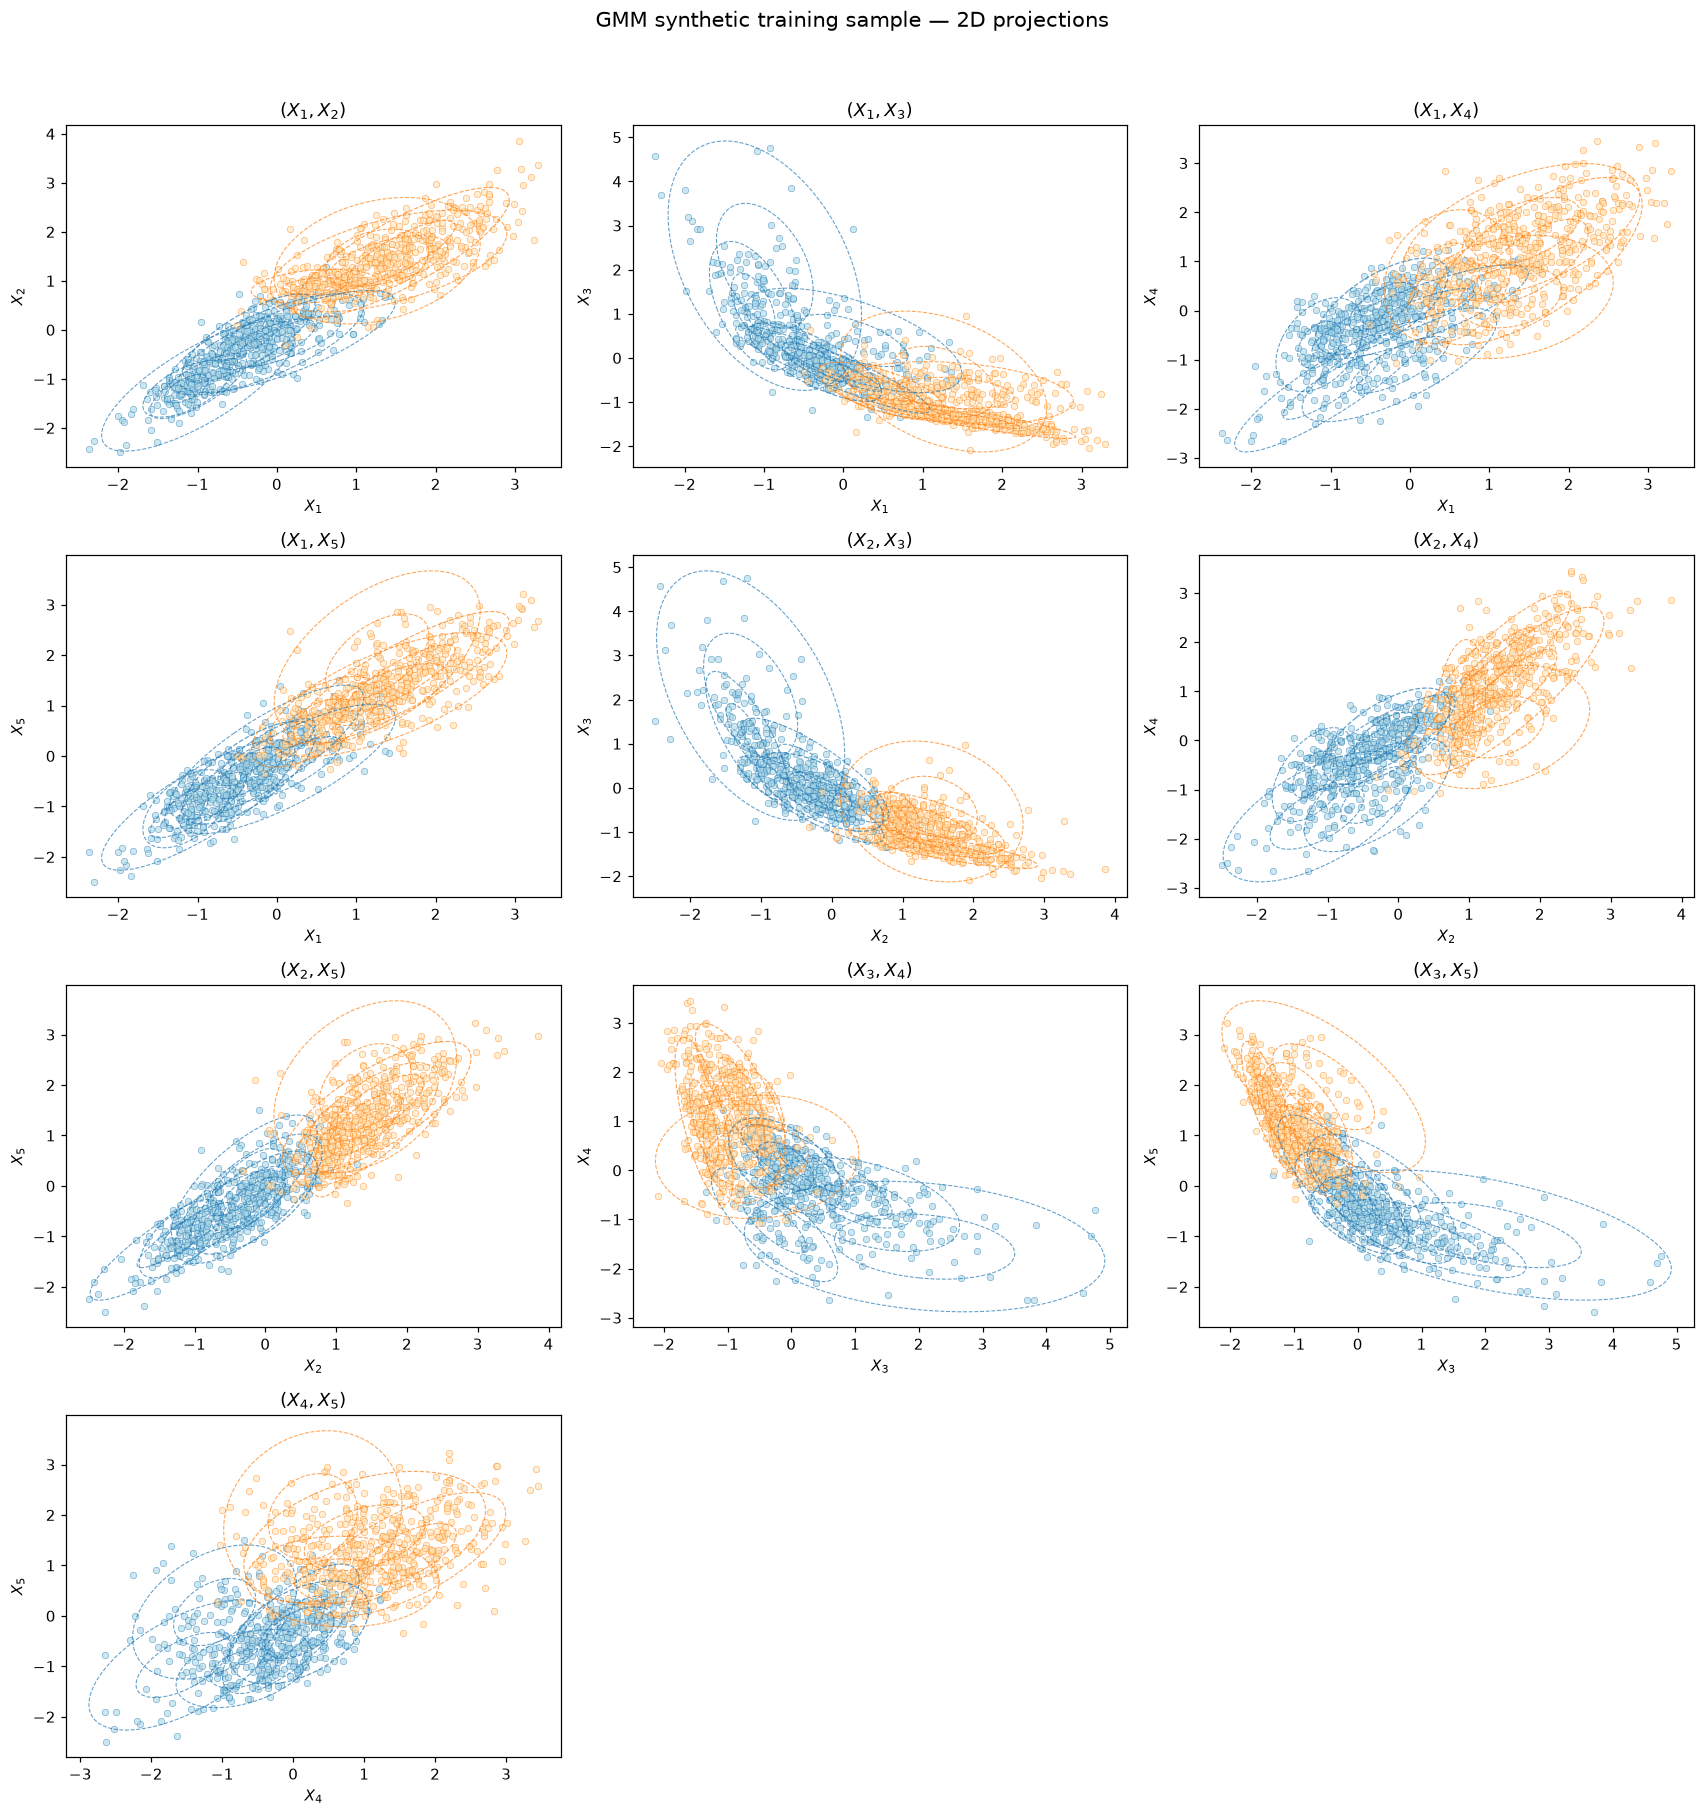
\includegraphics[width=\textwidth,height=0.82\textheight,keepaspectratio]{figures/geometry/air_quality/viz_2d_gmm_full_000005.png}
    \subcaption{GMM}
  \end{minipage}
  \sourcebelow{relatório publicado do cenário Air Quality 000005 do \CoInfoSim}
\end{figure}

\section{SUPPORT2}

\subsection{Origem e reformulação do alvo}

O SUPPORT foi um estudo multicêntrico sobre prognóstico, preferências e cuidados oferecidos a pacientes adultos gravemente enfermos \cite{support1995}. O modelo prognóstico associado estimou sobrevivência com base em informações clínicas disponíveis no início do acompanhamento \cite{knaus1995}. A versão pública SUPPORT2 utilizada neste trabalho é identificada pelo DOI \texttt{10.3886/ICPSR02957.v2}. O conjunto tornou-se um benchmark frequente em estudos de análise de sobrevivência e aprendizado de máquina, incluindo comparações entre modelos neurais, Cox e métodos de floresta de sobrevivência \cite{Kvamme2019Cox,Kvamme2019Continuous}.

O presente trabalho não reproduz integralmente uma tarefa de sobrevivência com censura. Foi derivado um alvo binário fixo de mortalidade em 180 dias:

\begin{equation}
  Y=\mathbb{1}\{\texttt{death}=1 \;\land\; \texttt{d.time}\leq 180\}.
  \label{eq:death180}
\end{equation}

O dia 180 é inclusivo. Pacientes com \texttt{death}=0 possuem acompanhamento superior ao horizonte no arquivo validado, permitindo a classificação binária sem rotular como sobrevivente um indivíduo cuja observação terminasse antes de 180 dias. Variáveis diretamente ligadas ao desfecho, como \texttt{death}, \texttt{d.time}, \texttt{hospdead}, \texttt{surv2m} e \texttt{surv6m}, são excluídas dos preditores.

\subsection{Canais e coorte de casos completos}

Foram utilizados sete canais fisiológicos basais:

\begin{enumerate}[label=$X_{\arabic*}$:]
  \item \texttt{meanbp}: pressão arterial média;
  \item \texttt{hrt}: frequência cardíaca;
  \item \texttt{resp}: frequência respiratória;
  \item \texttt{temp}: temperatura corporal;
  \item \texttt{wblc}: contagem de leucócitos;
  \item \texttt{crea}: creatinina;
  \item \texttt{sod}: sódio sérico.
\end{enumerate}

Com sete canais, são avaliados 127 subconjuntos não vazios. O arquivo original contém 9.105 pacientes, sendo 4.840 negativos e 4.265 positivos para o alvo derivado. A análise usa casos completos nos sete canais, nas duas variáveis necessárias ao alvo e no grupo diagnóstico \texttt{dzgroup}, empregado somente na estratificação e no relatório. A coorte final possui 8.873 pacientes, com 4.711 negativos e 4.162 positivos.

\subsection{Particionamento e padronização}

Foi construído um particionamento fixo 80/20 com semente 0 e estratificação conjunta por mortalidade em 180 dias e grupo diagnóstico. O reservatório de treinamento contém 7.098 pacientes, com 3.768 negativos e 3.330 positivos; o teste possui 1.775 pacientes, com 943 negativos e 832 positivos. Todos os 16 estratos conjuntos aparecem nas duas partições. Após o sorteio, as linhas são ordenadas pelo identificador, e os conjuntos são auditados por impressões digitais dos IDs.

A padronização utiliza somente o treinamento e $\mathrm{ddof}=0$. Não há imputação, transformação não linear ou recorte de valores. Essa escolha mantém o protocolo transparente, mas restringe as conclusões à coorte de casos completos e não equivale a uma recomendação clínica de exclusão de pacientes com exames ausentes.

\subsection{Geometria observada}

As projeções selecionadas do SUPPORT2 mostram regiões mais compatíveis com aproximações elipsoidais do que o Occupancy, ainda que as classes permaneçam fortemente sobrepostas. Essa combinação --- forma aproximadamente regular e baixa separabilidade --- é relevante para distinguir a dificuldade de classificar pacientes da capacidade de preservar relações relativas entre subconjuntos. O resultado do Random Forest, discutido posteriormente, torna essa distinção especialmente clara. A Figura~\ref{fig:geom-support2-dataset} apresenta as projeções bidimensionais dos sete canais fisiológicos nos três braços do cenário 000008.

\begin{figure}[H]
  \centering
  \caption{Geometrias padronizadas do cenário SUPPORT2}
  \label{fig:geom-support2-dataset}
  \begin{minipage}{\textwidth}
    \centering
    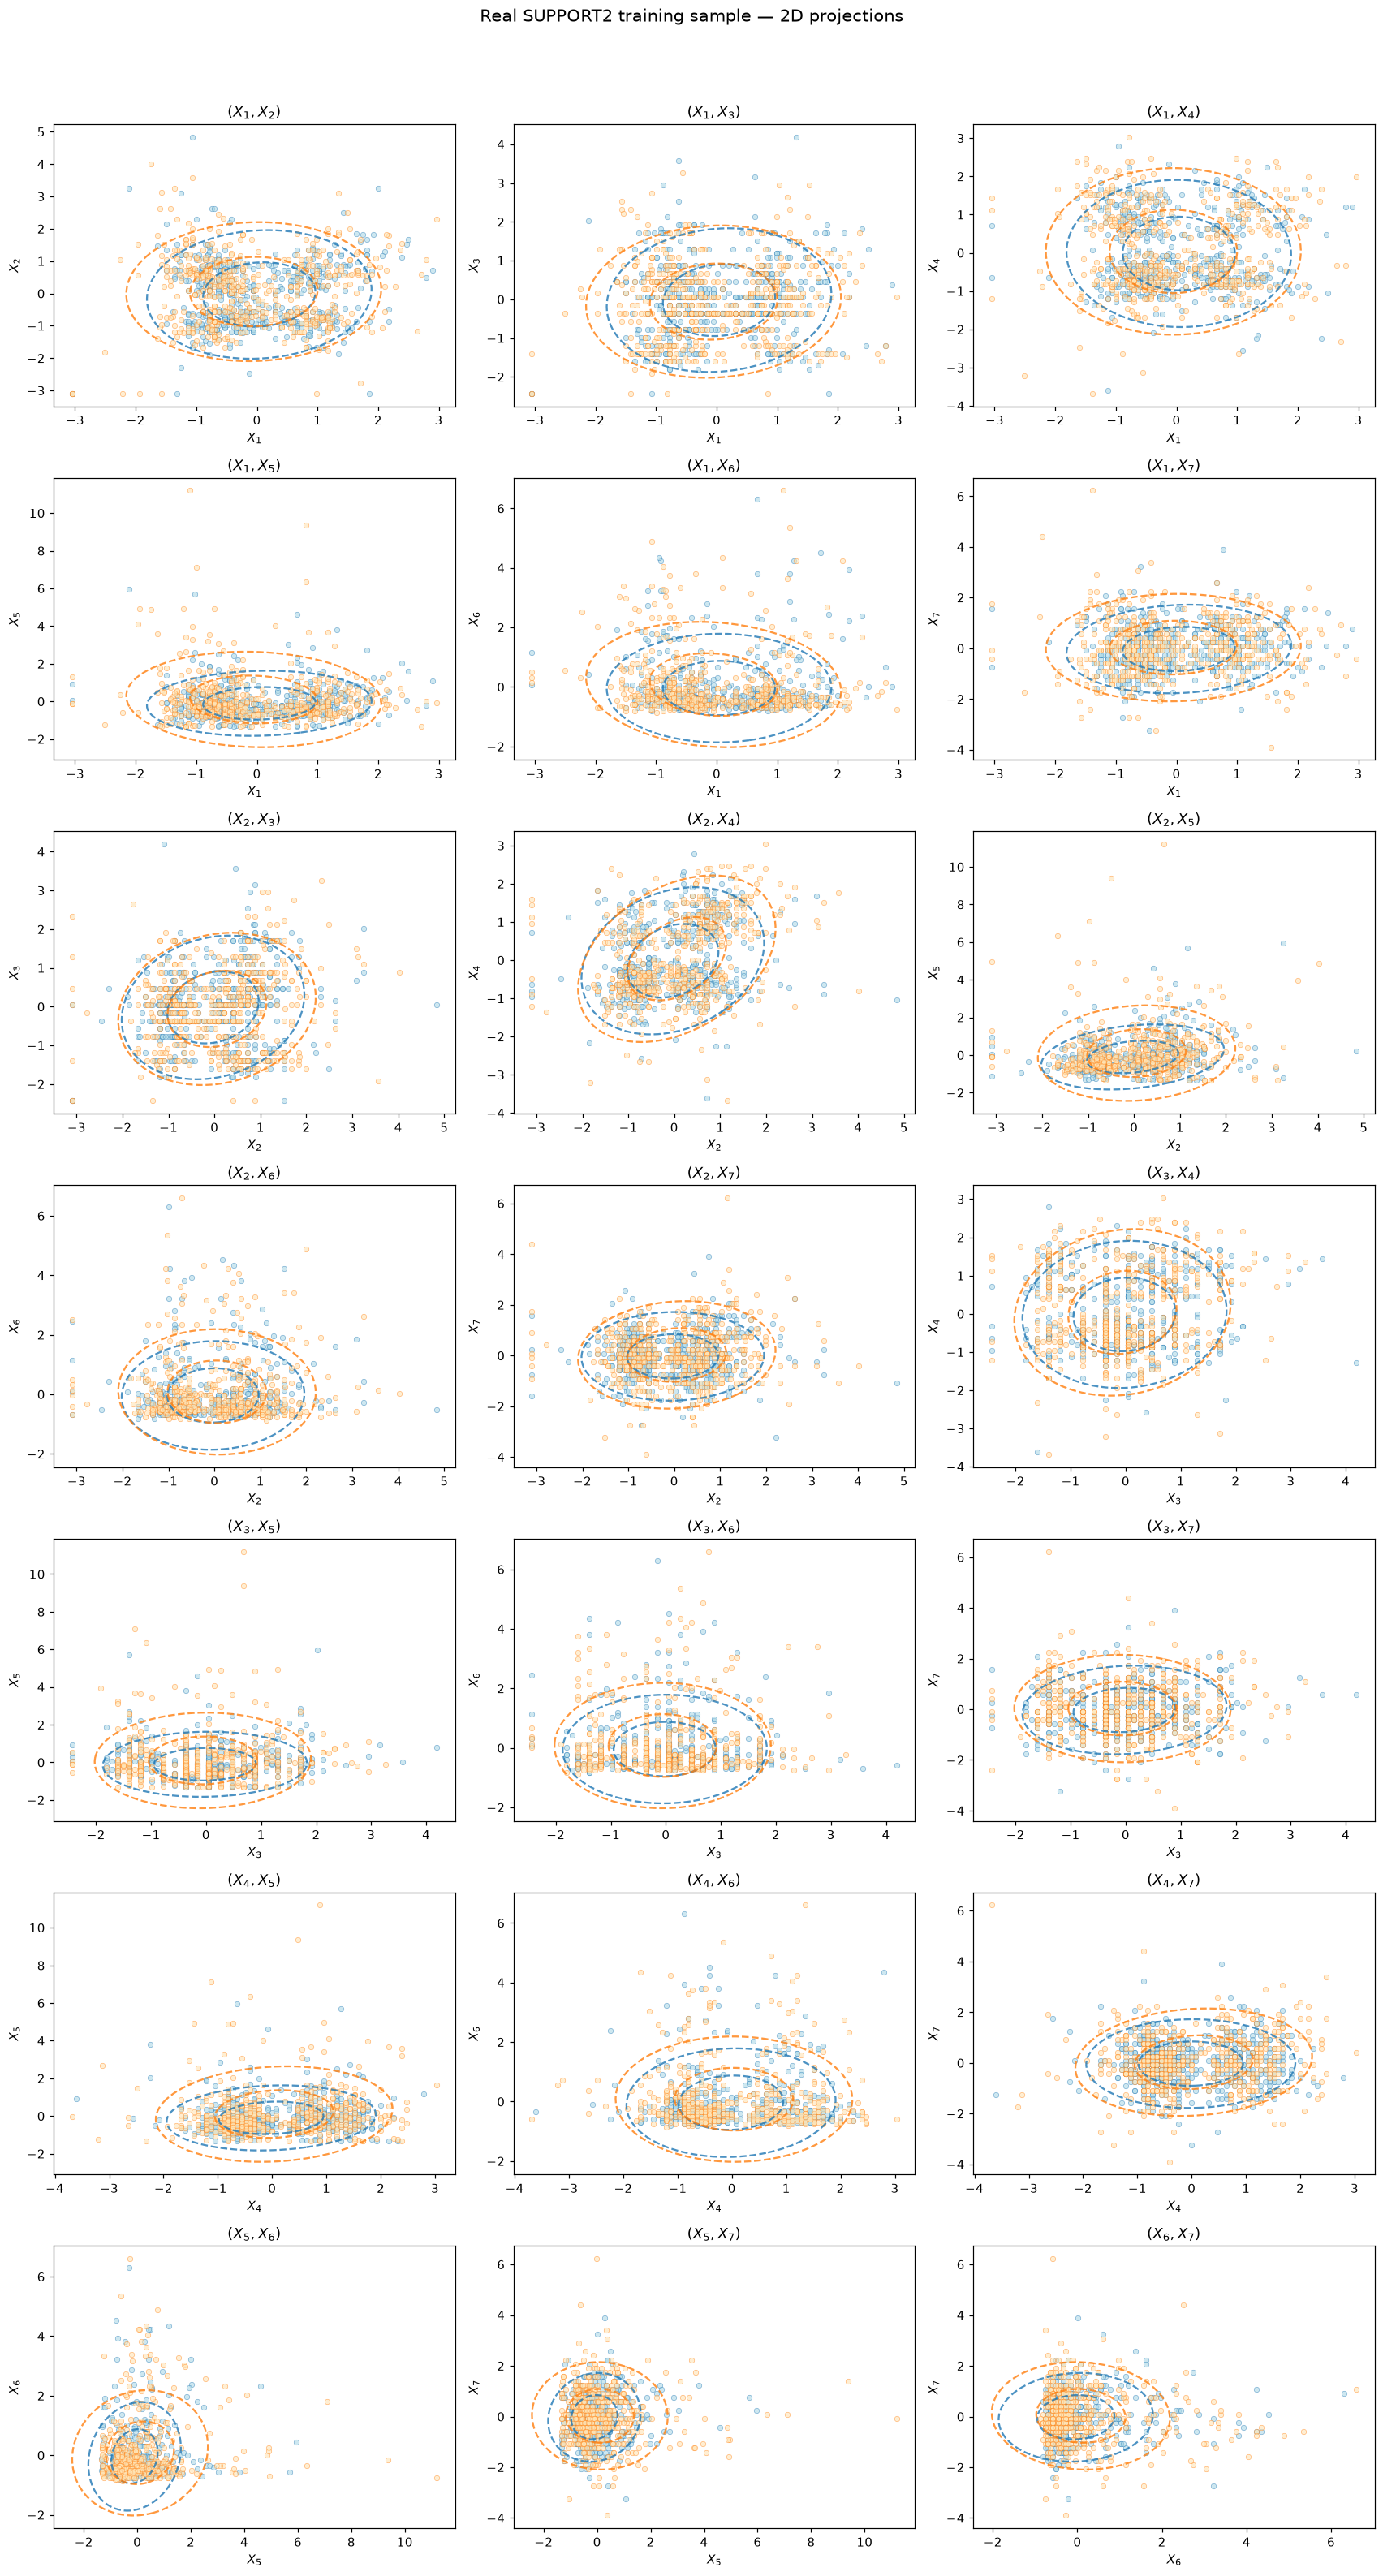
\includegraphics[width=\textwidth,height=0.80\textheight,keepaspectratio]{figures/geometry/support2/viz_2d_real_full_000008.png}
    \subcaption{Dados reais}
  \end{minipage}
  \sourcebelow{relatório publicado do cenário SUPPORT2 000008 do \CoInfoSim}
\end{figure}

\begin{figure}[H]
  \ContinuedFloat
  \centering
  \caption[]{Geometrias padronizadas do cenário SUPPORT2 (continuação)}
  \begin{minipage}{\textwidth}
    \centering
    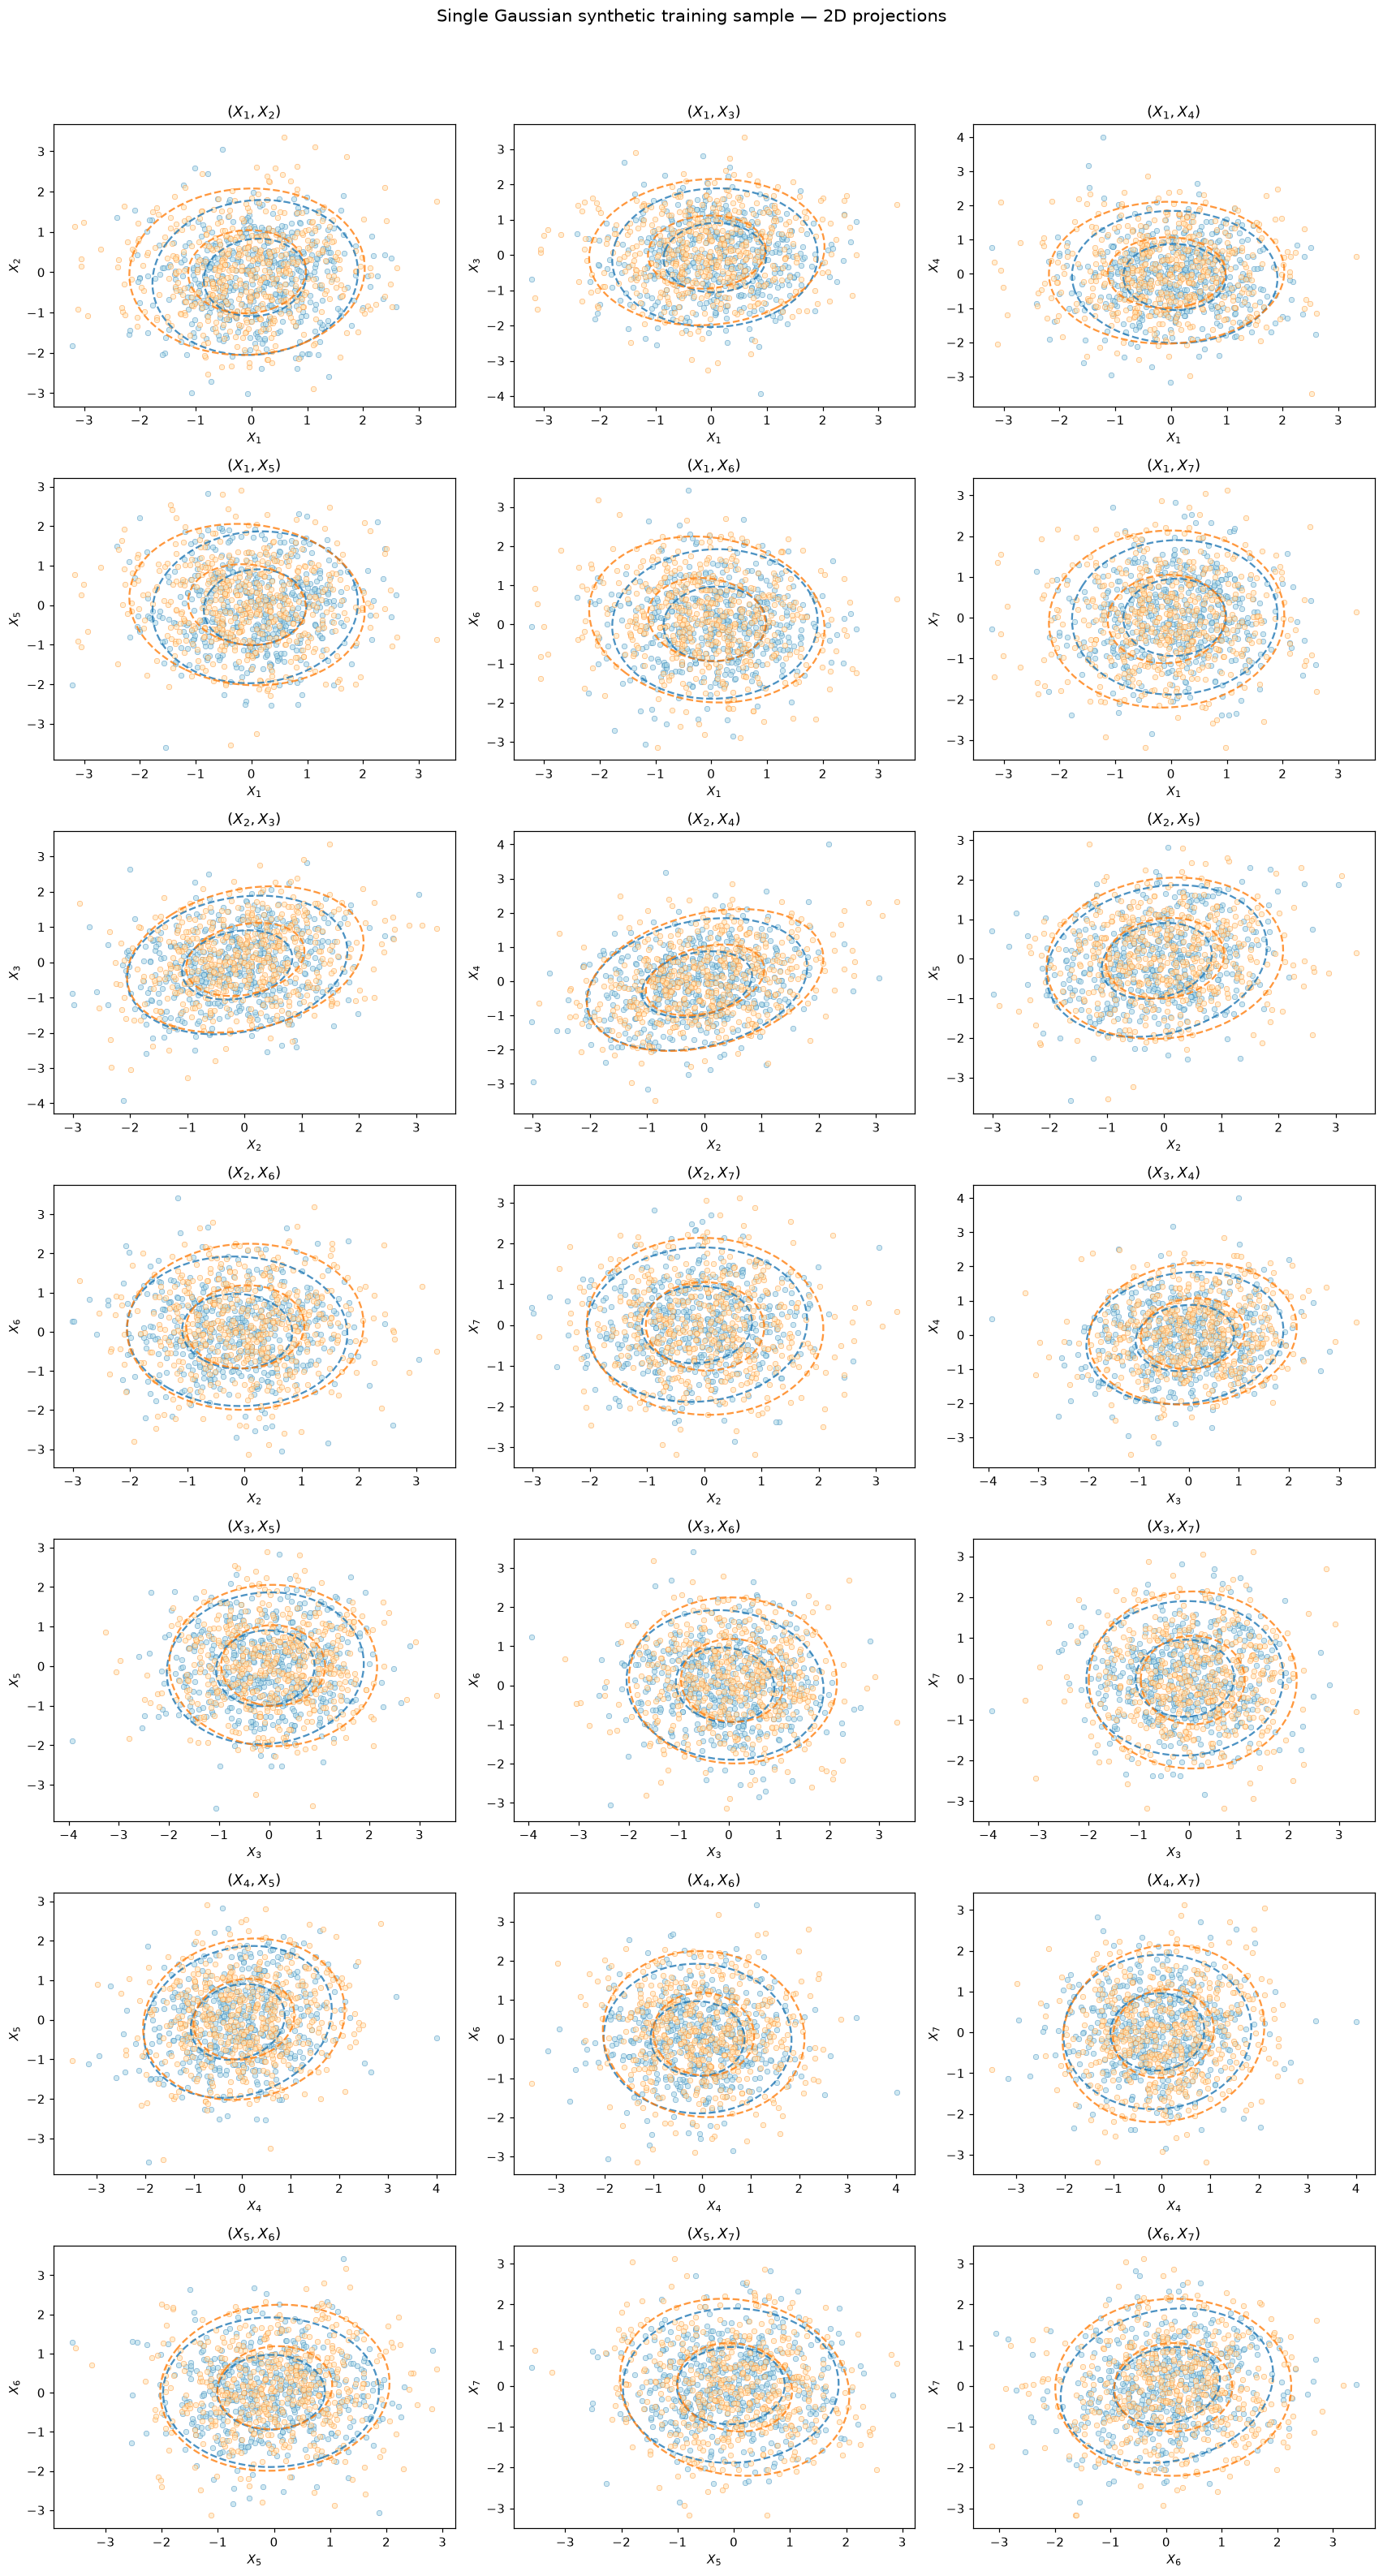
\includegraphics[width=\textwidth,height=0.80\textheight,keepaspectratio]{figures/geometry/support2/viz_2d_gaussian_full_000008.png}
    \subcaption{Gaussiana única}
  \end{minipage}
  \sourcebelow{relatório publicado do cenário SUPPORT2 000008 do \CoInfoSim}
\end{figure}

\begin{figure}[H]
  \ContinuedFloat
  \centering
  \caption[]{Geometrias padronizadas do cenário SUPPORT2 (continuação)}
  \begin{minipage}{\textwidth}
    \centering
    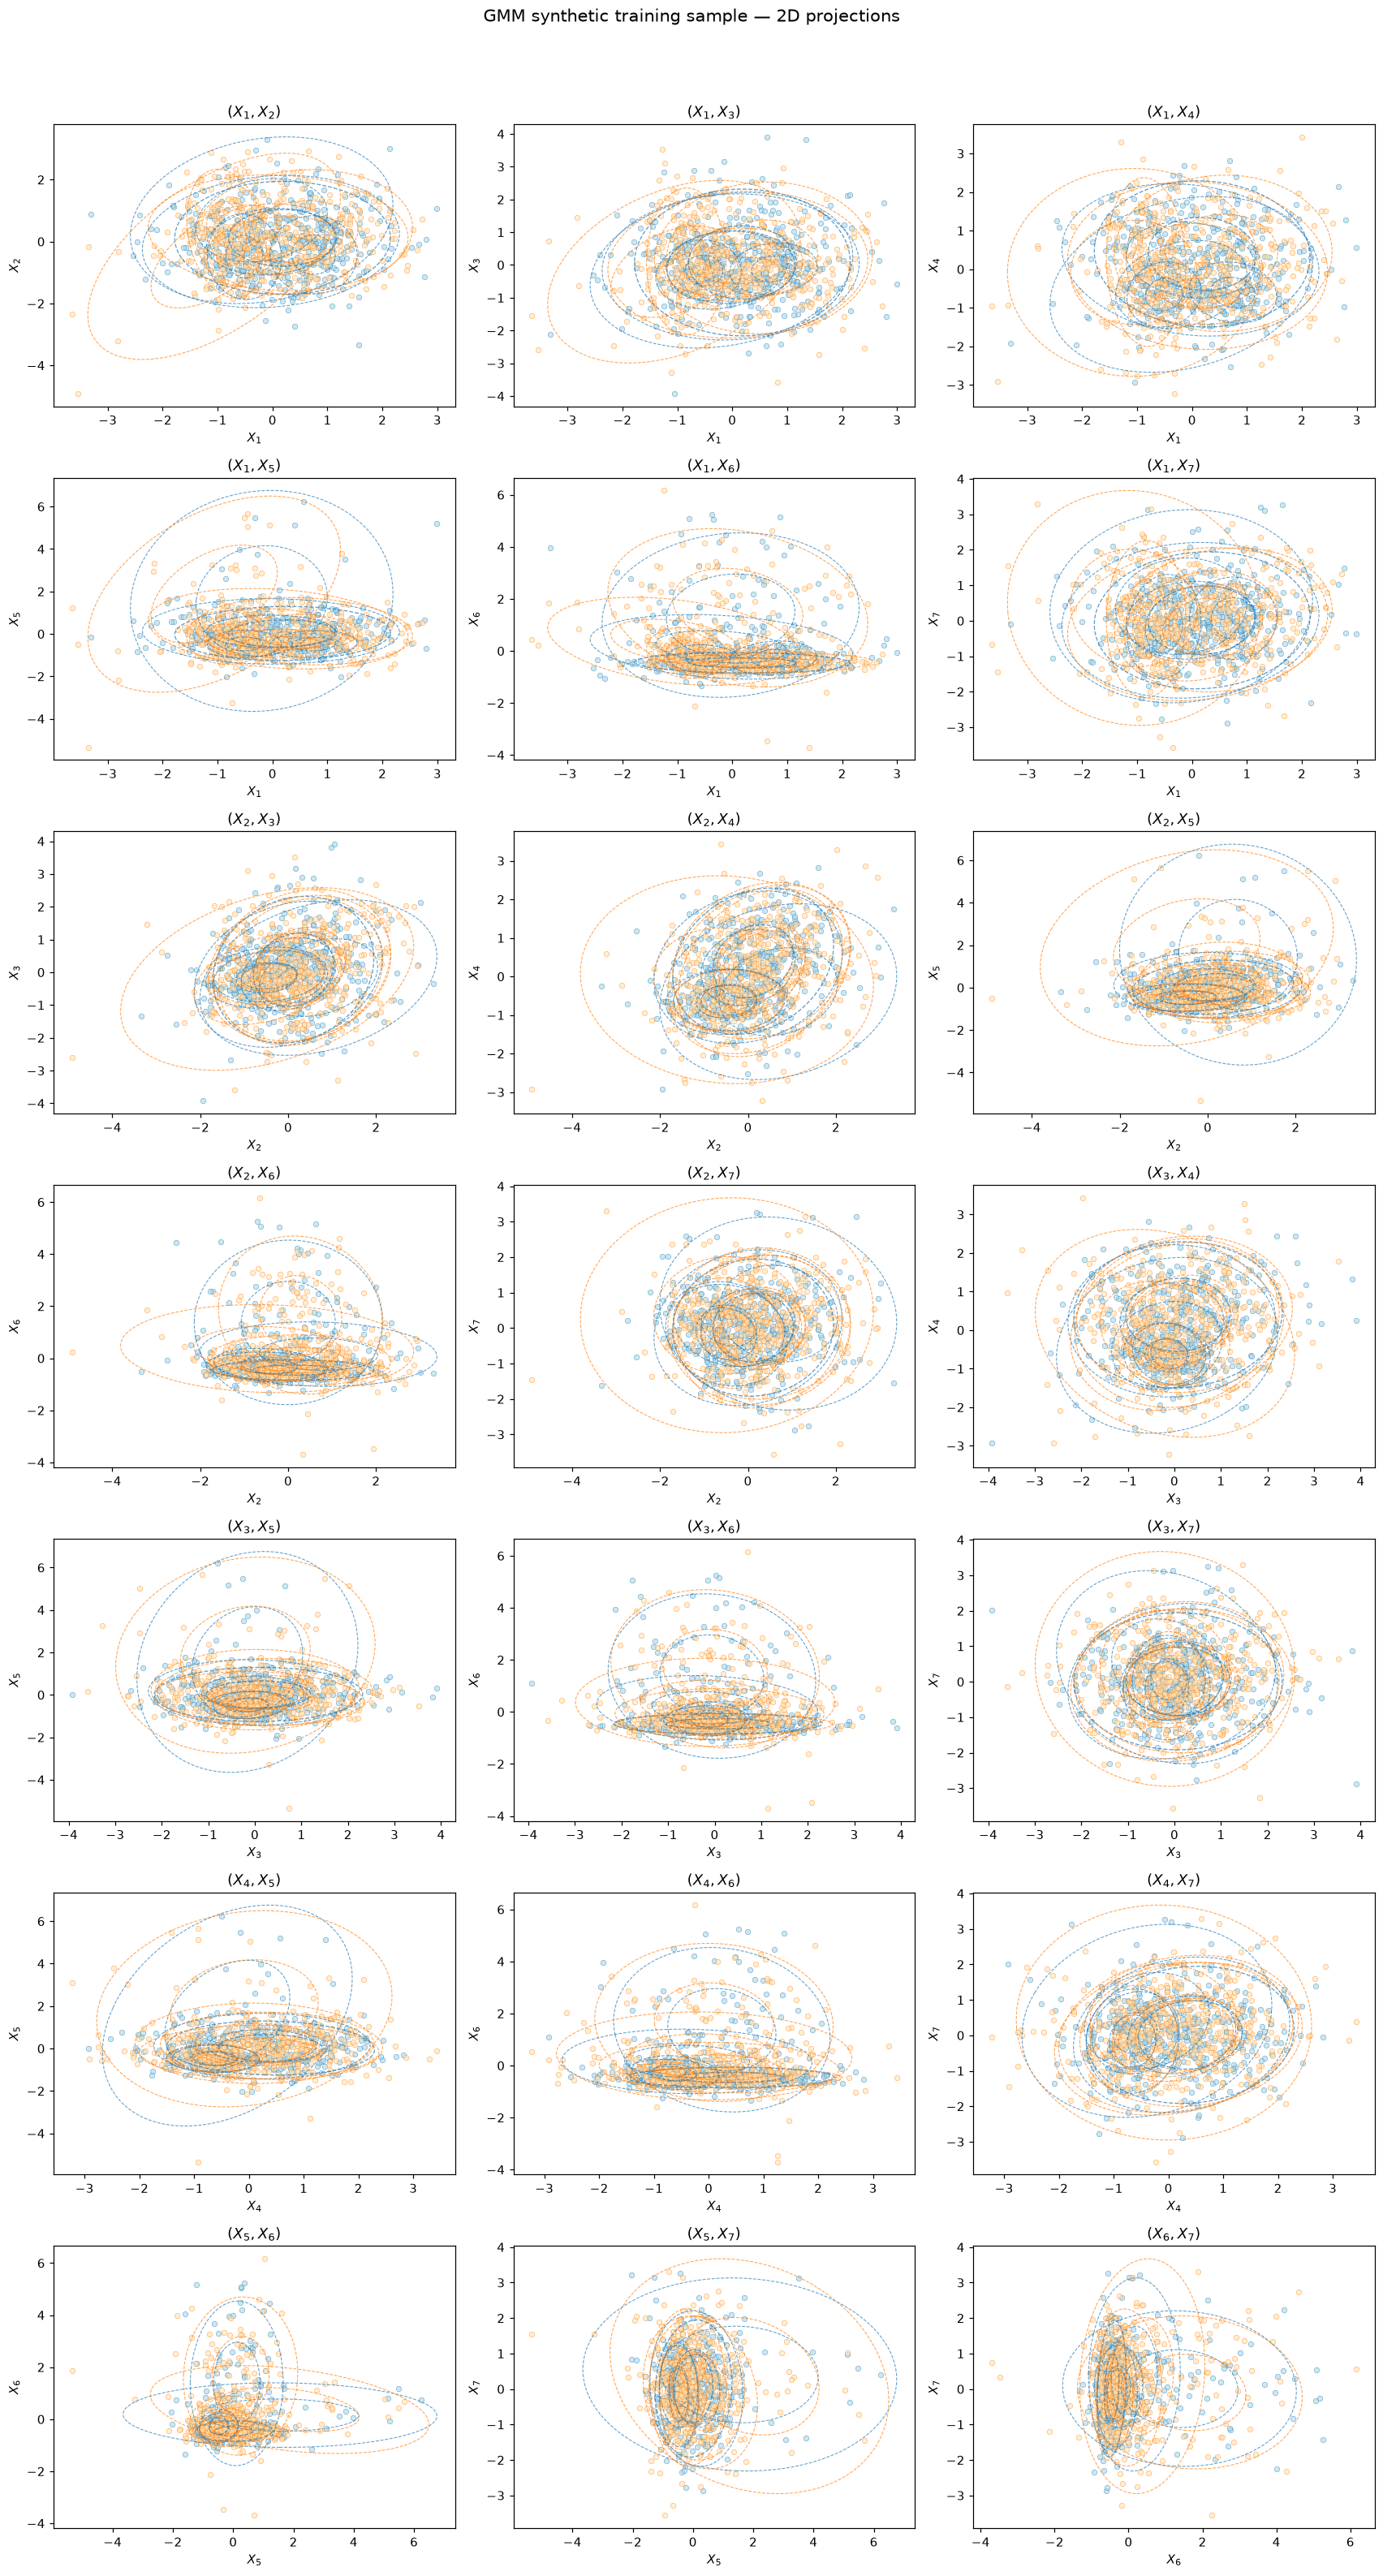
\includegraphics[width=\textwidth,height=0.80\textheight,keepaspectratio]{figures/geometry/support2/viz_2d_gmm_full_000008.png}
    \subcaption{GMM}
  \end{minipage}
  \sourcebelow{relatório publicado do cenário SUPPORT2 000008 do \CoInfoSim}
\end{figure}

\section{Síntese comparativa}

A Tabela \ref{tab:datasets-comparison} resume as diferenças que condicionam a interpretação dos resultados. Os três cenários compartilham avaliação exaustiva dos subconjuntos e teste real fixo, mas diferem na origem do alvo, na estrutura temporal e na quantidade de combinações. Consequentemente, a preservação estrutural não deve ser interpretada como atributo isolado do gerador: ela emerge da interação entre dataset, classificador, tamanho amostral e protocolo de avaliação.

\begin{table}[H]
  \centering
  \caption{Síntese dos datasets empregados no estudo}
  \label{tab:datasets-comparison}
  \begin{tabularx}{\textwidth}{>{\raggedright\arraybackslash}p{3.2cm}XXX}
    \toprule
    Propriedade & Occupancy & Air Quality & SUPPORT2 \\
    \midrule
    Domínio & Ambiente construído & Monitoramento ambiental & Prognóstico clínico \\
    Alvo & Ocupação da sala & Benzeno elevado, derivado da referência & Mortalidade em até 180 dias \\
    Canais & 5 & 5 & 7 \\
    Subconjuntos & 31 & 31 & 127 \\
    Reservatório de treinamento & 8.143 & 7.192 & 7.098 \\
    Teste real fixo & 12.417 & 1.799 & 1.775 \\
    Tipo de particionamento & Partição original do dataset & Cronológico 80/20 & Estratificado conjunto 80/20 \\
    Origem de $Y$ & Fotografias marcadas no tempo & Analisador de referência excluído de $X$ & Evento e tempo de acompanhamento \\
    Geometria exploratória & Fortemente não gaussiana & Mais regular e aproximadamente elipsoidal & Aproximadamente elipsoidal, com forte sobreposição \\
    \bottomrule
  \end{tabularx}
  \sourcebelow{elaboração própria}
\end{table}
